%\documentclass[10pt,a4paper]{article}
\documentclass[nojss]{jss}

\usepackage[utf8]{inputenc}

%\usepackage{a4wide}
\usepackage{amsfonts}
%\setlength{\parskip}{0.5ex plus0.1ex minus0.1ex}
%\setlength{\parindent}{0em}

%\usepackage[round,longnamesfirst]{natbib}
%\usepackage{hyperref}
%\usepackage{verbatim}
%%% for tabulars
%\usepackage{rotating}
%\usepackage{multirow}


%\newcommand{\strong}[1]{{\normalfont\fontseries{b}\selectfont #1}}
\newcommand{\class}[1]{\mbox{\textsf{#1}}}
\newcommand{\func}[1]{\mbox{\texttt{#1()}}}
%\newcommand{\code}[1]{\mbox{\texttt{#1}}}
%\newcommand{\pkg}[1]{\strong{#1}}
\newcommand{\samp}[1]{`\mbox{\texttt{#1}}'}
%\newcommand{\proglang}[1]{\textsf{#1}}
\newcommand{\set}[1]{\mathcal{#1}}

\newcommand{\mat}[1]{\mathbf{#1}}

%\usepackage{Sweave}
%% \VignetteIndexEntry{Visualizing Association Rules: Introduction to arulesViz}

%\title{Visualizing Association Rules: Introduction to the R-extension Package \pkg{arulesViz}}

\author{Michael Hahsler\\Southern Methodist University \And
	Sudheer Chelluboina\\Southern Methodist University}
\title{Visualizing Association Rules: Introduction to the R-extension Package \pkg{arulesViz}}
%% for pretty printing and a nice hypersummary also set:
\Plainauthor{Michael Hahsler, Sudheer Chelluboina} %% comma-separated
\Plaintitle{Visualizing Association Rules: Introduction to the R-extension Package rulesViz}
\Shorttitle{Visualizing Association Rules} %% a short title (if necessary)

%% an abstract and keywords
\Abstract{
Association rule mining is a popular data mining method available in R as the
extension package~\pkg{arules}.  However, mining association rules often results
in a very large number of found rules, leaving the analyst with the task to go
through all the rules and discover interesting ones. Sifting manually through
large sets of rules is time consuming and strenuous. Visualization has a long
history of making large data sets better accessible using techniques like
selecting and zooming. In this paper we present the R-extension
package~\pkg{arulesViz} which implements several known and novel visualization
techniques to explore association rules.
With examples we show how these visualization techniques can be used to analyze a data set.
    }
\Keywords{data mining, association rules, visualization}
\Plainkeywords{data mining, association rules, visualization} %% without formatting


\Address{
    Michael Hahsler\\
    Engineering Management, Information, and Systems\\
    Lyle School of Engineering\\
    Southern Methodist University\\
    P.O. Box 750123 \\
    Dallas, TX 75275-0123\\
    E-mail: \email{mhahsler@lyle.smu.edu}\\
    URL: \url{http://lyle.smu.edu/~mhahsler}
}




\begin{document}
%% ------------------------------------------------------------------
%% ------------------------------------------------------------------
%\title{Visualizing Association Rules: Introduction to the R-extension Package \pkg{arulesViz}}
%\author{Michael Hahsler and Sudheer Chelluboina}
\maketitle
\sloppy
%% ------------------------------------------------------------------
%% ------------------------------------------------------------------
%\begin{abstract}
%Association rule mining is a popular data mining method available in R as the
%extension package~\pkg{arules}.  However, mining association rule often results
%in a very large number of found rules, leaving the analyst with the task to go
%through all the rules and discover interesting ones. Sifting manually through
%large sets of rules is time consuming and strenuous. Visualization has a long
%history of making large data sets better accessible using techniques like
%selecting and zooming. In this paper we present the R-extension
%package~\pkg{arulesViz} which implements several known and novel visualization
%techniques to explore association rules.
%With examples we show how these visualization techniques can be used to analyze a data set.
%\end{abstract}

%% ------------------------------------------------------------------
%% ------------------------------------------------------------------
%\clearpage
%\tableofcontents
%\clearpage
%% ------------------------------------------------------------------
%% ------------------------------------------------------------------

\section{Introduction}

Many organizations generate a large amount of transaction data
on a daily basis.
For example, a
department store like ``Macy's'' stores customer shopping information at a
large scale using check-out data.  Association rule mining is one of the major
techniques to detect and extract useful information from large scale transaction
data. Mining association rules
was fist introduced by ~\cite{arules:Agrawal+Imielinski+Swami:1993}
and can formally be defined as:

Let $I=\{i_1, i_2,\ldots,i_n\}$ be a set of $n$ binary attributes called
\emph{items}.  Let $\set{D} = \{t_1, t_2, \ldots, t_m\}$ be a set of
transactions called the \emph{database}. Each transaction in~$\set{D}$ has an
unique transaction ID and contains a subset of the items in~$I$.  A \emph{rule}
is defined as an implication of the form $X \Rightarrow Y$ where $X, Y
\subseteq I$ and $X \cap Y = \emptyset$.  The sets of items (for short
\emph{itemsets}) $X$ and $Y$ are called \emph{antecedent} (left-hand-side or
LHS) and \emph{consequent} (right-hand-side or RHS) of the rule.
Often rules are restricted to only a single item in the consequent.

\emph{Association rules} are rules which surpass a user-specified
minimum support
and minimum confidence threshold. The \emph{support}~$\mathrm{supp}(X)$ of an itemset~$X$
is defined as the proportion of transactions in the data set which contain the
itemset and the \emph{confidence} of a rule is defined
$\mathrm{conf}(X\Rightarrow Y) = \mathrm{supp}(X \cup Y) / \mathrm{supp}(X)$.
Therefore, an association rule $X\Rightarrow Y$ will satisfy:
$$\mathrm{supp}(X\cup Y) \ge \sigma$$
and
$$\mathrm{conf}(X\Rightarrow Y) \ge \delta$$
where $\sigma$ and $\delta$ are the minimum support and minimum confidence,
respectively.

Another popular measure for association rules used throughout this paper
is \emph{lift}~\citep{arules:Brin+Motwani+Ullman+Tsur:1997}.
The lift of a rule is defined as
$$\mathrm{lift}(X \Rightarrow Y) = \mathrm{supp}(X\cup Y)/(\mathrm{supp}(X)\mathrm{supp}(Y))$$
and can be interpreted as the deviation of the support of the whole
rule from the support expected under independence given the supports
of both sides of the rule.
Greater lift values ($\gg 1$) indicate stronger associations.
Measures like support, confidence and lift are generally called
interest measures because they help with focusing on
potentially more interesting rules.


For a more detailed treatment of association rules we refer the reader to
the in introduction paper for package~\pkg{arules}
\citep{arulesViz:Hahsler:2010, arulesViz:Hahsler:2005}
and the literature referred to there.

Association rules are typically generated in a two-step process. First, minimum
support is used to generate the set of all {\em frequent itemsets} for the data
set. Frequent itemsets are itemsets which satisfy the minimum support
constraint. Then, in a second step, each frequent itemsets is used to generate
all possible rules from it and all rules which do not satisfy the minimum
confidence constraint are removed.
Analyzing this process, it is easy to see that in
the worst case we will generate
$2^n-n-1$ frequent itemsets
with more than two items
from a database with $n$ distinct items.
%Then, if we restrict oursleves to single-item consequents, we can generate a
%maximum of
%$$\sum_{k=2}^{n}k\binom{n}{k} = n(2^{n-1}-1)$$
%\marginpar{check}
Since each frequent itemset will in the worst case generate at least two rules,
we will end up with a set of rules in the order of $O(2^n)$.
Typically, increasing minimum support is used to keep the number of association
rules found at a manageable size. However, this also removes potentially
interesting rules with less support. Therefore, the need to deal with
large sets of association rules is
unavoidable when applying association rule mining in a real setting.

Visualization is successfully used to communicate both abstract and concrete
ideas in many areas like education, engineering and
science~\citep{arulesViz:Prangsmal:2009}.
According to \cite{arulesViz:Chen:2008}, the application of visualization
falls into two phases.
First, the exploration phase where the
analysts will use graphics that are mostly incompatible for presentation
purposes but make it easy to find interesting and important features
of the data. The amount of interaction needed during exploration is very high
and includes filtering, zooming and rearranging data.
After key findings are discovered in the data, these findings must be presented
in a way suitable for presentation for a larger audience.
In this second phase it is important that the analyst can manipulate the
presentation to clearly highlight the findings.

Many researchers introduced visualization techniques
like scatter plots, matrix visualizations, graphs, mosaic plots
and parallel coordinates plots to analyze association rules
(see \cite{arulesViz:Bruzzese:2008} for a recent overview paper).
This paper discusses existing techniques and
demonstrates how their implementation in \pkg{arulesViz}
can be used via a simple unified interface.
We extend most plots using techniques of color shading and reordering to
improve their interpretability.
Finally, this paper also introduces a completely new method
called ``grouped matrix-based visualization'' which is based on a novel
way of clustering rules.
Clustering rules is usually based on distances defined on the items included
in the rules or on shared transactions covered by the rules. However,
here we cluster rules especially for visualization using similarities between
sets of values of a selected interest measure.

The rest of the paper is organized as follows.
In Section~\ref{sec:prep} we give a very short example
of how to prepare data using package~\pkg{arules} and then introduce
the unified interface provided by~\pkg{arulesViz} for association
rule visualization.
In Sections~\ref{sec:scatter} to \ref{sec:doubledecker} we describe
the different visualization techniques and give examples.
Most of the techniques are enhanced using color shading and reordering.
Grouped matrix-based visualization in Section~\ref{sec:grouped} is
a novel visualization technique.
In Section~\ref{sec:comp} compares the presented visualization techniques.
Section~\ref{sec:conclusion} concludes the paper.


\section{Data preparation and unified interface of arulesViz}
\label{sec:prep}

To use \pkg{arulesViz} we fist have to load the package.
The package automatically loads other needed packages like
\pkg{arules}~\citep{arulesViz:Hahsler:2010}
for handling and mining association rules.
For the examples in this paper we load
the ``Groceries'' data set which is included in \pkg{arules}.

\begin{Schunk}
\begin{Sinput}
> library("arulesViz")
> data("Groceries")
\end{Sinput}
\end{Schunk}

Groceries contains sales data from a local grocery store with 9835 transactions
and 169 items (product groups). The summary shows some basic statistics of
the data set. For example, that the data set is rather sparse
with a density just above 2.6\%, that
``whole milk'' is the most popular item and that the average transaction
contains less than 5 items.

\begin{Schunk}
\begin{Sinput}
> summary(Groceries)
\end{Sinput}
\begin{Soutput}
transactions as itemMatrix in sparse format with
 9835 rows (elements/itemsets/transactions) and
 169 columns (items) and a density of 0.02609146 

most frequent items:
      whole milk other vegetables       rolls/buns             soda 
            2513             1903             1809             1715 
          yogurt          (Other) 
            1372            34055 

element (itemset/transaction) length distribution:
sizes
   1    2    3    4    5    6    7    8    9   10   11   12   13   14   15 
2159 1643 1299 1005  855  645  545  438  350  246  182  117   78   77   55 
  16   17   18   19   20   21   22   23   24   26   27   28   29   32 
  46   29   14   14    9   11    4    6    1    1    1    1    3    1 

   Min. 1st Qu.  Median    Mean 3rd Qu.    Max. 
  1.000   2.000   3.000   4.409   6.000  32.000 

includes extended item information - examples:
       labels  level2           level1
1 frankfurter sausage meat and sausage
2     sausage sausage meat and sausage
3  liver loaf sausage meat and sausage
\end{Soutput}
\end{Schunk}

Next we mine association rules using the Apriori algorithm implemented
in \pkg{arules}.

\begin{Schunk}
\begin{Sinput}
> rules <- apriori(Groceries, parameter=list(support=0.001, confidence=0.5))
\end{Sinput}
\begin{Soutput}
Apriori

Parameter specification:
 confidence minval smax arem  aval originalSupport maxtime support minlen
        0.5    0.1    1 none FALSE            TRUE       5   0.001      1
 maxlen target   ext
     10  rules FALSE

Algorithmic control:
 filter tree heap memopt load sort verbose
    0.1 TRUE TRUE  FALSE TRUE    2    TRUE

Absolute minimum support count: 9 

set item appearances ...[0 item(s)] done [0.00s].
set transactions ...[169 item(s), 9835 transaction(s)] done [0.00s].
sorting and recoding items ... [157 item(s)] done [0.00s].
creating transaction tree ... done [0.00s].
checking subsets of size 1 2 3 4 5 6 done [0.01s].
writing ... [5668 rule(s)] done [0.00s].
creating S4 object  ... done [0.00s].
\end{Soutput}
\begin{Sinput}
> rules
\end{Sinput}
\begin{Soutput}
set of 5668 rules 
\end{Soutput}
\end{Schunk}

The result is a set of 5668 association rules.
The top three rules
with respect to the lift measure,
a popular measure of rule strength, are:

\begin{Schunk}
\begin{Sinput}
> inspect(head(sort(rules, by ="lift"),3))
\end{Sinput}
\begin{Soutput}
    lhs                             rhs              support    
[1] {Instant food products,soda} => {hamburger meat} 0.001220132
[2] {soda,popcorn}               => {salty snack}    0.001220132
[3] {flour,baking powder}        => {sugar}          0.001016777
    confidence lift    
[1] 0.6315789  18.99565
[2] 0.6315789  16.69779
[3] 0.5555556  16.40807
\end{Soutput}
\end{Schunk}

However, it is clear that going through all the 5668 rules
manually is not a viable
option. We therefore will introduce different visualization techniques
implemented in~\pkg{arulesViz}.
All implemented visualization techniques share the
following interface:

\begin{Schunk}
\begin{Sinput}
> plot(x, method = NULL, measure = "support", shading = "lift",
+   interactive = FALSE, data = NULL, control = NULL, ...)
\end{Sinput}
\end{Schunk}

where \code{x} is the set of rules to be visualized,
\code{method} is the visualization method,
\code{measure} and \code{shading} contain the interest measures
used by the plot,
\code{interactive} indicates if we want to interactively
explore or just present the rules,
\code{data} can contain the transaction data set used to mine the
rules (only necessary for some methods) and \code{control} is a list
with further control arguments to customize the plot.

In the following sections we will introduce the different visualization
methods implemented in \pkg{arulesViz} and demonstrate how easy it is to
use them.

\section{Scatter plot}
\label{sec:scatter}

A straight-forward visualization of association rules is to use a scatter plot
with two interest measures on the axes.
Such a presentation can be found already in an early paper by
\cite{arulesViz:Bayardo:1999} when they discuss \emph{sc-optimal rules.}

The default method for \func{plot} for association rules
in \pkg{arulesViz}
is a scatter plot using support and confidence on the axes.
In addition a third measure (default: lift) is used as the color (gray level)
of the points. A color key is provided to the right of the plot.

\begin{Schunk}
\begin{Sinput}
> plot(rules)
\end{Sinput}
\end{Schunk}

\begin{figure}
\centering
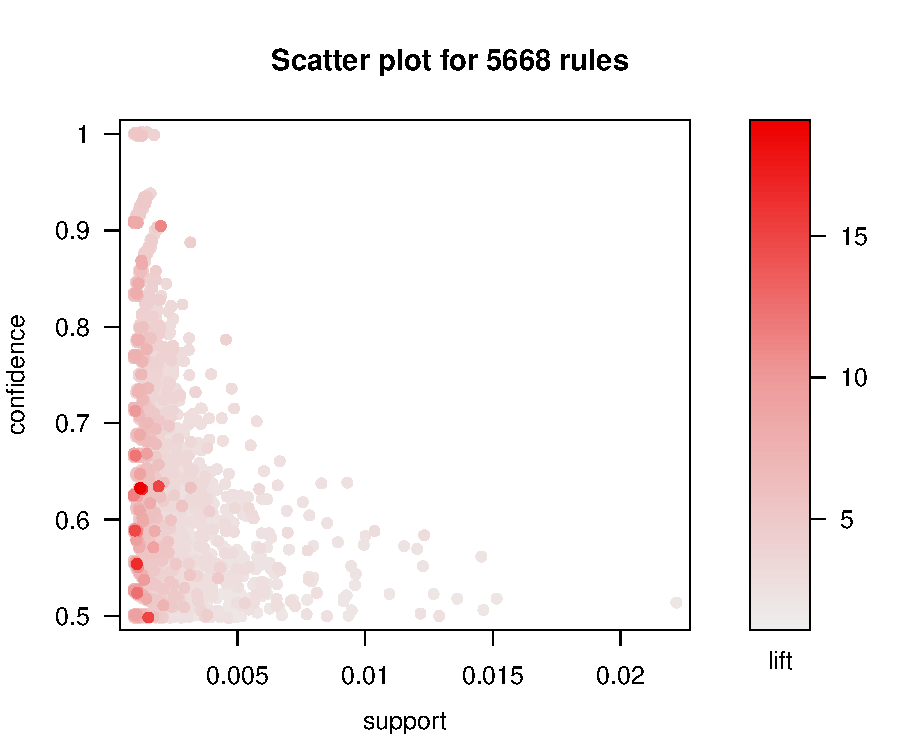
\includegraphics[width=10cm]{arulesViz-scatterplot1}
\caption{Default scatter plot.\label{fig:scatterplot1}}
\end{figure}

This plot for the rules mined in the previous section is shown in
Figure~\ref{fig:scatterplot1}. We can see
that rules with high lift
have typically a relatively low support.
\cite{arulesViz:Bayardo:1999} argue that
the most interesting rules (sc-optimal rules)
reside on the support/confidence border, which can be clearly seen in this
plot. We will show later how the interactive features of this
plot can be used to explore these rules.

Any measure stored in the quality slot of the set of rules can be used
for the axes (vector of length 2 for parameter \code{measure})
or for color shading~(\code{shading}).
The following measures are available for our set of
rules.
\begin{Schunk}
\begin{Sinput}
> head(quality(rules))
\end{Sinput}
\begin{Soutput}
      support confidence     lift
1 0.001118454  0.7333333 2.870009
2 0.001220132  0.5217391 2.836542
3 0.001321810  0.5909091 2.312611
4 0.001321810  0.5652174 2.212062
5 0.001321810  0.5200000 2.035097
6 0.003660397  0.6428571 2.515917
\end{Soutput}
\end{Schunk}

These are the default measures generated by Apriori. To add other measures
we refer the reader to the function \func{interestMeasure}
included in \pkg{arules}.
For example we can customize the plot by switching lift and confidence:

\begin{Schunk}
\begin{Sinput}
> plot(rules, measure=c("support", "lift"), shading="confidence")
\end{Sinput}
\end{Schunk}

Figure~\ref{fig:scatterplot2} shows this plot with lift on the y-axis. Here it
is easy to identify all rules with high lift.

\begin{figure}
\centering
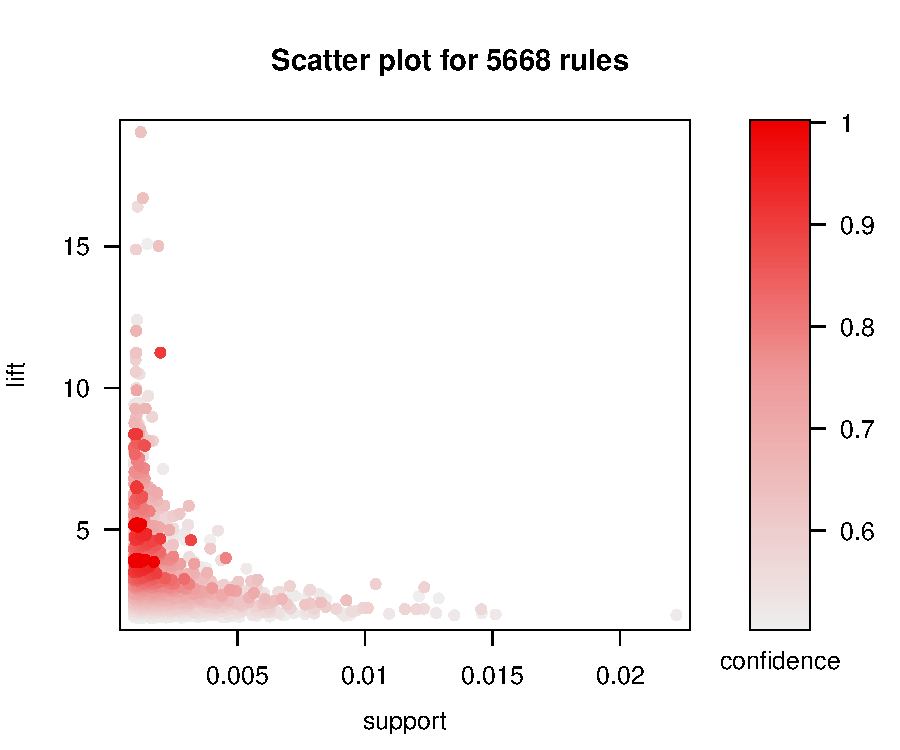
\includegraphics[width=10cm]{arulesViz-scatterplot2}
\caption{Scatter plot with lift on the y-axis.\label{fig:scatterplot2}}
\end{figure}

\cite{arulesViz:Unwin:2001} introduced a special version of a scatter plot
called \emph{Two-key plot.} Here support and confidence are used for the x and
y-axes and the color of the points is used to indicate ``order,'' i.e.,
the number of items contained in the rule. Two-key plots can be produced
using the unified interface by:

\begin{Schunk}
\begin{Sinput}
> plot(rules, shading="order", control=list(main = "Two-key plot"))
\end{Sinput}
\end{Schunk}

\begin{figure}
\centering
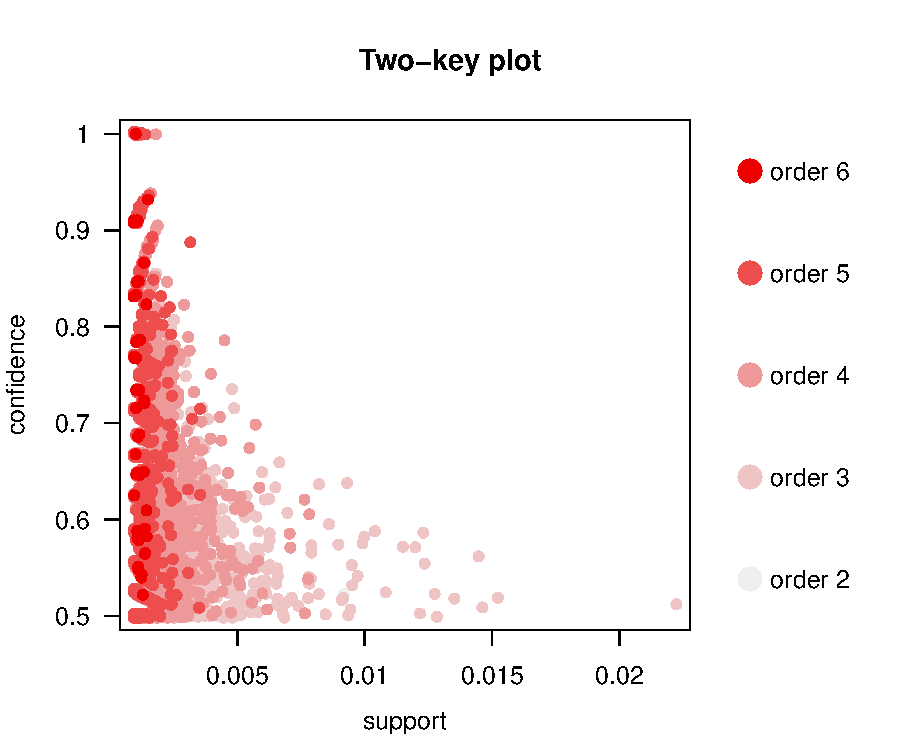
\includegraphics[width=10cm]{arulesViz-scatterplot3}
\caption{Two-key plot.\label{fig:scatterplot3}}
\end{figure}

The resulting Two-key plot is shown in Figure~\ref{fig:scatterplot3}.
From the plot it is clear that order and support have a very strong
inverse relationship, which is a known fact for association rules
\citep{arulesViz:Seno:2005}.


In addition to using order for shading, we also give the plot a different
title (\code{main}).
Other control options including \code{pch} (best with filled symbols: 20--25),
\code{cex}, \code{xlim} and \code{ylim} are available and work in the
usual way expected by R-users.

For exploration,
the scatter plot method offers interactive features for selecting
and zooming. Interaction
is activated using \code{interactive=TRUE}.

\begin{Schunk}
\begin{Sinput}
> sel <- plot(rules, measure=c("support", "lift"), shading="confidence", interactive=TRUE)
\end{Sinput}
\end{Schunk}

Interactive features include:
\begin{itemize}
\item Inspecting individual rules by selecting them and clicking the
inspect button.
\item Inspecting sets of rules
by selecting a rectangular region of the plot and clicking the
inspect button.
\item Zooming into a selected region (zoom in/zoom out buttons).
\item Filtering rules using the measure used for shading
by clicking the filter button and selecting a cut-off point
in the color key. All rules with a measure lower than the cut-off
point will be filtered.
\item Returning the last selection for further analysis (end button).
\end{itemize}

%% fixme - new screenshot
\begin{figure}
\centering
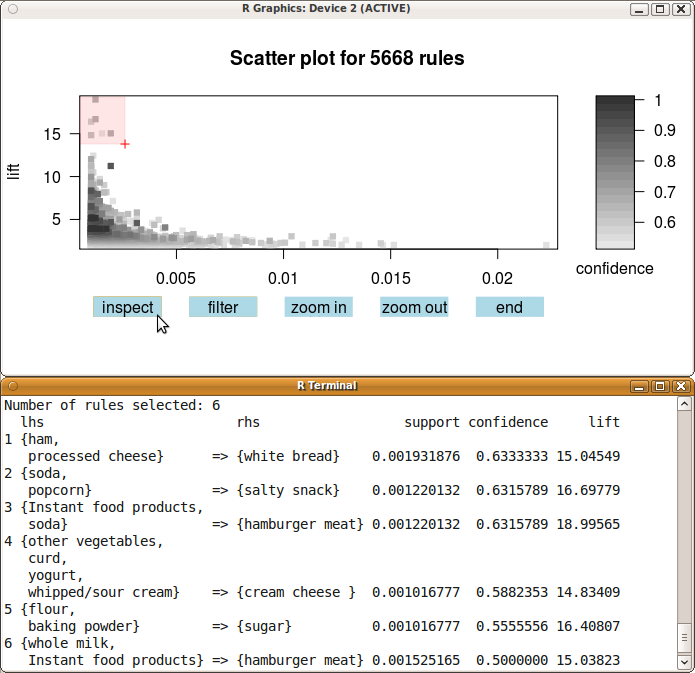
\includegraphics[width=11cm]{scatterplot_interactive.png}
\caption{Interactive mode for scatter plot (inspecting rules with
high lift).\label{fig:interaction}}
\end{figure}

The result of an
example interaction is shown in Figure~\ref{fig:interaction}.
Using a box selection the rules with the highest lift are selected. Using the
inspect button, the rules are displayed in the terminal below the plotting
device.

\section{Matrix-based visualizations}
\label{sec:matrix-based}
Matrix-based visualization techniques organize the
antecedent and consequent itemsets
on the x and y-axes, respectively. A selected interest measure
is displayed at the intersection of the antecedent and
consequent of a given rule. If no rule is available for a
antecedent/consequent combination the intersection area is left blank.

Formally, the visualized matrix is constructed as follows.
We start with the set of association rules
$$\set{R} = \{
    \langle a_1,c_1,m_1\rangle, \ldots
    \langle a_i,c_i,m_i\rangle, \ldots
    \langle a_n,c_n,m_n\rangle\}$$
where $a_i$ is the antecedent, $c_i$ is the consequent and $m_i$ is the
selected interest measure
for the $i$-th rule for $i = 1,\ldots,n$.
    In $\set{R}$ we identify the set of $K$ unique
antecedents and $L$ unique consequent. We create a $L \times K$ matrix
$\mat{M}$ with one column for each unique antecedent and one row for each
unique consequent.  Finally, we populate the matrix by setting
$\mat{M}_{lk} = m_i$ for $i=1,\ldots,n$ and $l$ and $k$ corresponding
to the position of $a_i$ and $c_i$ in the matrix.
Note that $\mat{M}$ will contain many empty cells since
many potential association rules
will not meet the required minimum thresholds on
support and confidence.

\cite{arulesViz:Ong:2002} presented a version of the
matrix-based visualization
technique where a 2-dimensional matrix is used and the interest measure
is represented by color shading of squares at the
intersection.
An alternative visualization option is to use 3D bars at the intersection
\citep{arulesViz:Wong:1999,arulesViz:Ong:2002}.

For this type of visualization the number of rows/columns depends on the
number of unique itemsets in the consequent/antecedent in the set of
rules. Since large sets of rules typically have a large number
of different itemsets as antecedents (often not much smaller than the number of rules themselves), the size of the colored squares
or the 3D bars gets very small and hard to see.
We reduce the number of
rules here by filtering out all rules with a low confidence score.

\begin{Schunk}
\begin{Sinput}
> subrules <- rules[quality(rules)$confidence > 0.8]
> subrules
\end{Sinput}
\begin{Soutput}
set of 371 rules 
\end{Soutput}
\end{Schunk}

\begin{Schunk}
\begin{Sinput}
> plot(subrules, method="matrix", measure="lift")
\end{Sinput}
\end{Schunk}

The resulting plot is shown in Figure~\ref{fig:matrix1}.
Since there is not much space
for long labels in the plot, we only show numbers as
labels for rows and columns and the complete itemsets are printed to
the terminal for look-up. We omit the complete output here,
since this plot and the next few plots print several hundred labels
to the screen. The output looks like:

\begin{verbatim}
Itemsets in Antecedent (lhs)
  [1] "{liquor,red/blush wine}"
  [2] "{curd,cereals}"
  [3] "{yogurt,cereals}"
  [4] "{butter,jam}"
  [5] "{soups,bottled beer}"
	    (lines omitted)
  [343] "{tropical fruit,root vegetables,rolls/buns,bottled water}"
  [344] "{tropical fruit,root vegetables,yogurt,rolls/buns}"
Itemsets in Consequent (rhs)
  [1] "{bottled beer}"     "{whole milk}"       "{other vegetables}"
  [4] "{tropical fruit}"   "{yogurt}"           "{root vegetables}"
\end{verbatim}

The visual impression can be improved by
reordering rows and columns in the matrix
such that rules with similar values of the interest measure are presented
closer together.
This removes some of the fragmentation in the
matrix display and therefore makes it easier to see structure.

\begin{Schunk}
\begin{Sinput}
> plot(subrules, method="matrix", measure="lift", control=list(reorder=TRUE))
\end{Sinput}
\end{Schunk}

In the resulting plot in Figure~\ref{fig:matrix2} we
see the emergence of two large
blocks of rules with two different consequents and then smaller blocks
for the rest. With the interactive mode (\code{interactive=TRUE})
colored squares can be selected
and the rule it represents will be displayed on the screen.
This can
be used to explore different antecedents which have a similar impact on
the same consequent in terms of the measure used in the plot.

Reordering is done using the \pkg{seriation}
package~\citep{arulesViz:Hahsler:2008} which provides a wide array of
ordering methods for multivariate data. Typically, finding the optimal
order subject to some defined objective function
is a difficult combinatorial optimization problem which involves
for $n$ objects to check many of the $O(n!)$ possible permutations.
However, for visualization purposes
some suboptimal but fast heuristics are acceptable and it is
often sufficient to try several methods to find the most useful representation.
However, it is useful to understand the different methods
and the objective function they try to optimize.
Some available useful methods are:
\begin{itemize}
\item "PCA" -- First principal component. Uses the first principal component
for the data matrix and for the transposed matrix as order for
    rows and columns. This is a very fast approach which avoids the expensive
    distance matrix computation.

\item "TSP" -- Traveling salesperson problem solver. Computes distance matrices
    between rows and between columns and solves two separate TSPs. By default
    the nearest insertion heuristic is used. This method is reasonably fast for
    small rule sets, but the distance matrix computation and the associated
    memory requirements make it impractical for larger sets.

\item "HC" -- Hierarchical clustering. Computes distance matrices
    for rows and columns and
    then clusters twice. Distance matrix computation is again limiting
    the approach for smaller sets.

\item "max", "avg" and "median" -- Reorder rows/columns by their maximum,
    average or median value. This extremely simple and fast methods
    provides sometimes good visualizations.
\end{itemize}

Other available methods include "BEA", "MDS", "OLO", "GW", "ARSA" and "BBURCG".
We refer the interested reader to \cite{arulesViz:Hahsler:2008} for
detailed description of these methods.
Different seriation
methods can be selected via \code{reorderMethod} in the control list
(default: TSP). For the methods which first compute dissimilarity matrices,
the control list argument \code{reorderDist} can be used to specify the
used measure (default: Euclidean distance).

Most seriation methods cannot handle missing values.
However, the visualized matrix typically contains many missing values since
minimum support discards of many rules during rule mining.  We use a very crude
imputation approach by replacing the missing values in the matrix (values for
rules not contained in the rules set) by a fixed value (0 by default).

\begin{figure}
\centering
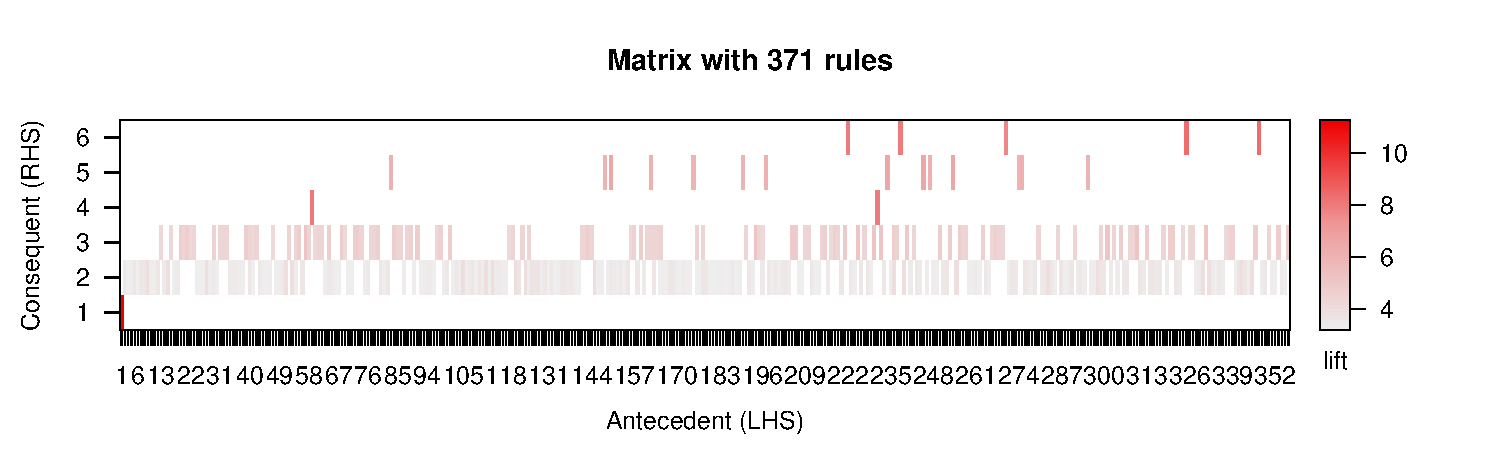
\includegraphics[width=\linewidth]{arulesViz-matrix1}
\caption{Matrix-based visualization with colored squares.
\label{fig:matrix1}}

\vspace{5mm}

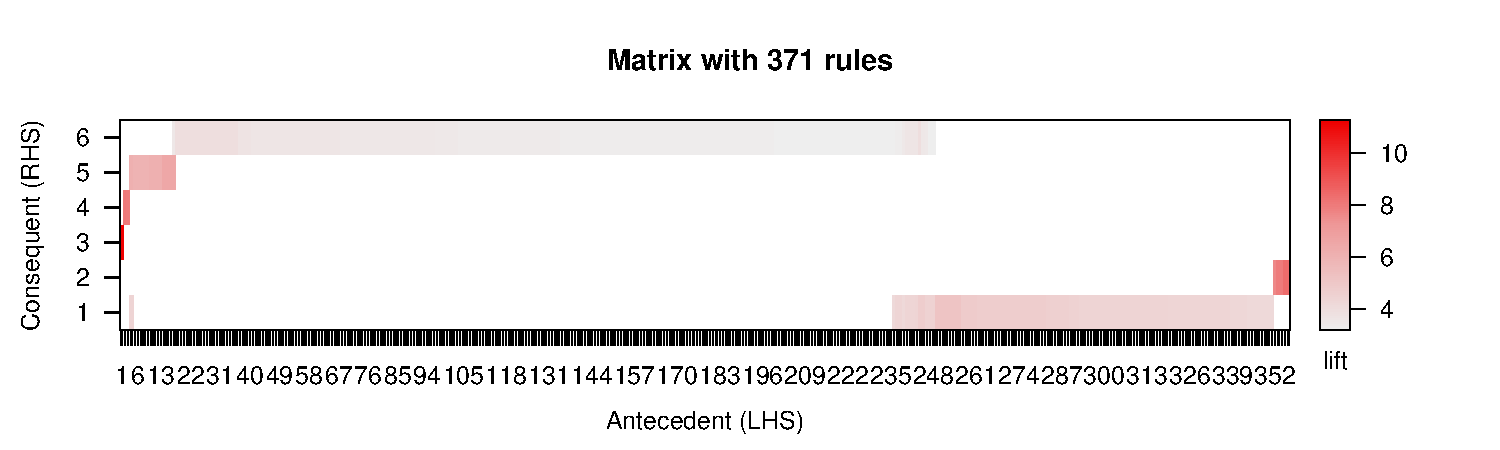
\includegraphics[width=\linewidth]{arulesViz-matrix2}
\caption{Matrix-based visualization with colored squares (reordered).
\label{fig:matrix2}}
\end{figure}


An alternative representation is to use
3D bars (method ``matrix3D'') instead of colored rectangles.

\begin{Schunk}
\begin{Sinput}
> plot(subrules, method="matrix3D", measure="lift")
\end{Sinput}
\end{Schunk}
\begin{Schunk}
\begin{Sinput}
> plot(subrules, method="matrix3D", measure="lift", control=list(reorder=TRUE))
\end{Sinput}
\end{Schunk}

\begin{figure}
\begin{minipage}{.48\linewidth}
\centering
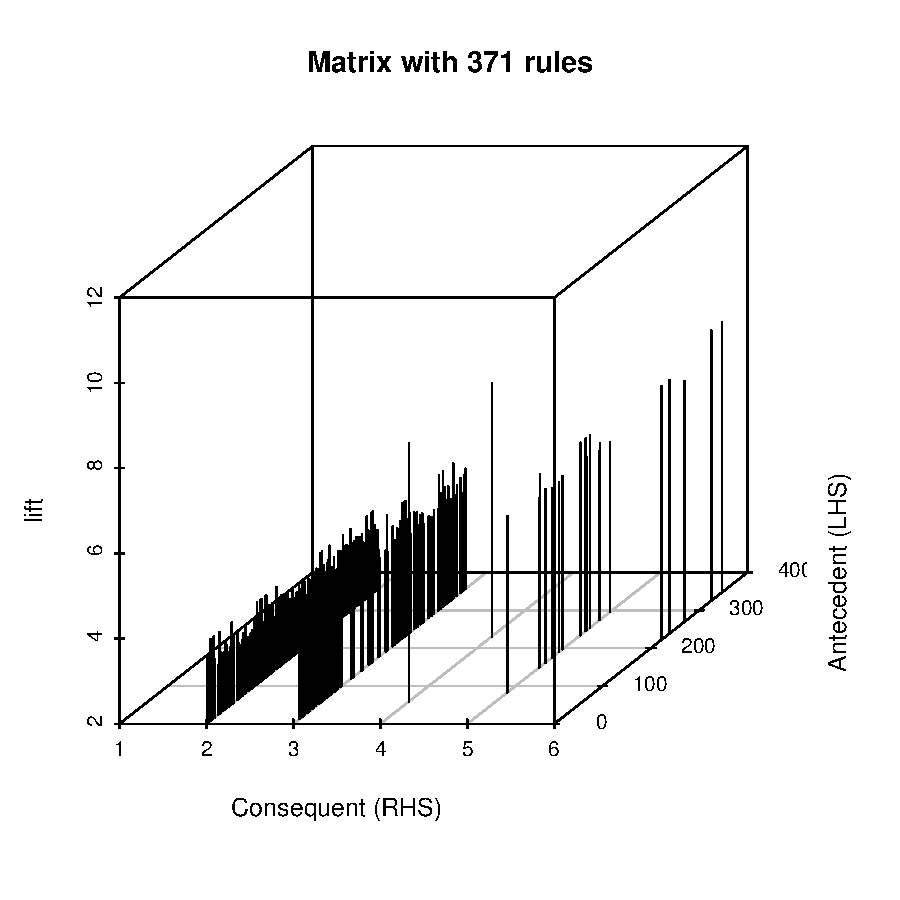
\includegraphics[width=\linewidth]{arulesViz-matrix3D1}
\caption{Matrix-based visualization with 3D bars.
\label{fig:matrix3D1}}
\end{minipage}
\begin{minipage}{.48\linewidth}
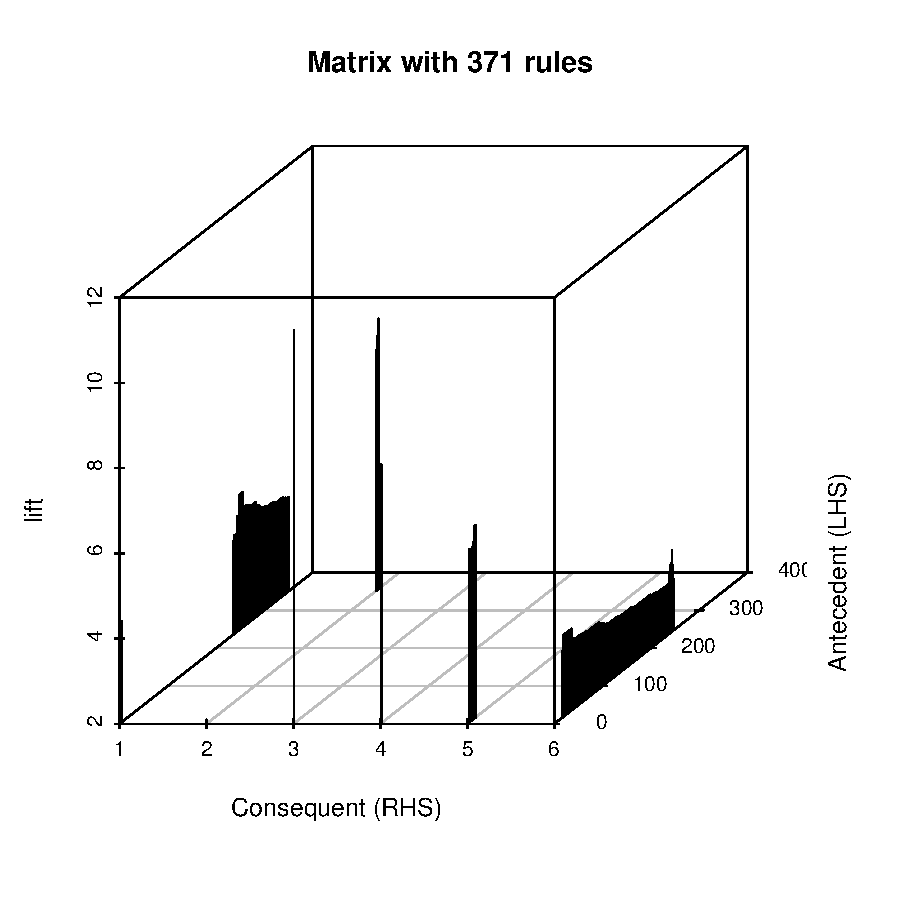
\includegraphics[width=\linewidth]{arulesViz-matrix3D2}
\caption{Matrix-based visualization with 3D bars (reordered).
\label{fig:matrix3D2}}
\end{minipage}
\end{figure}

The 3D visualization is shown in Figures~\ref{fig:matrix3D1} and
\ref{fig:matrix3D2}.

If we specify a vector with two measures, both measures
are used simultaneously using color hue for one measure and luminance
and chroma together for the other.

\begin{Schunk}
\begin{Sinput}
> plot(subrules, method="matrix", measure=c("lift", "confidence"))
\end{Sinput}
\end{Schunk}
\begin{Schunk}
\begin{Sinput}
> plot(subrules, method="matrix", measure=c("lift", "confidence"),
+         control=list(reorder=TRUE))
\end{Sinput}
\end{Schunk}

\begin{figure}
\centering
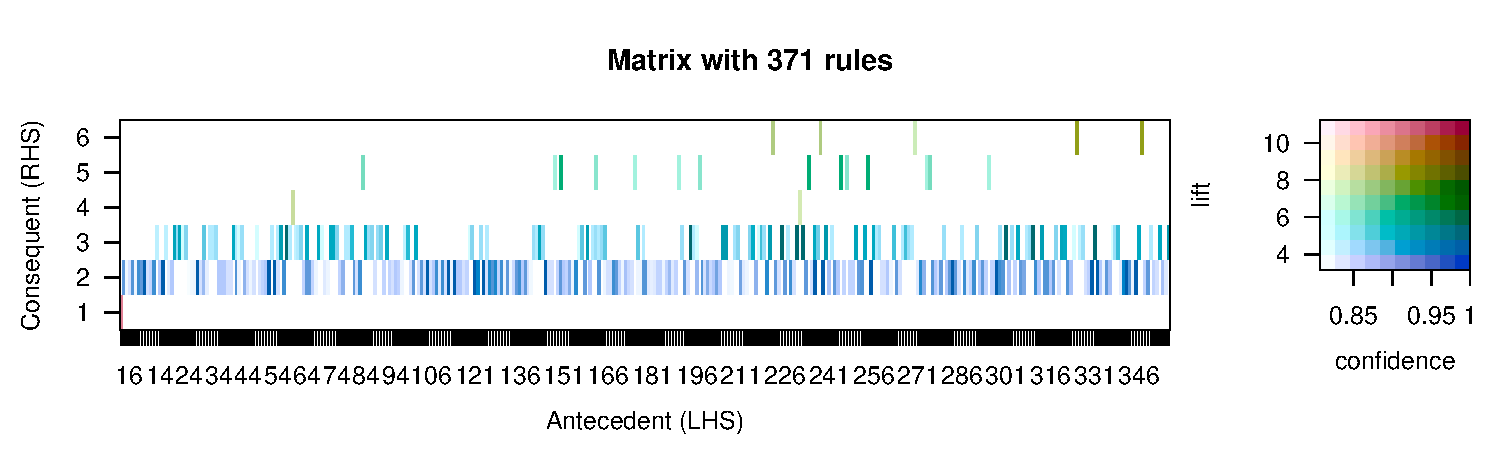
\includegraphics[width=\linewidth]{arulesViz-matrix_col1}
\caption{Matrix-based visualization of two measures with colored squares.
\label{fig:matrix_col1}}

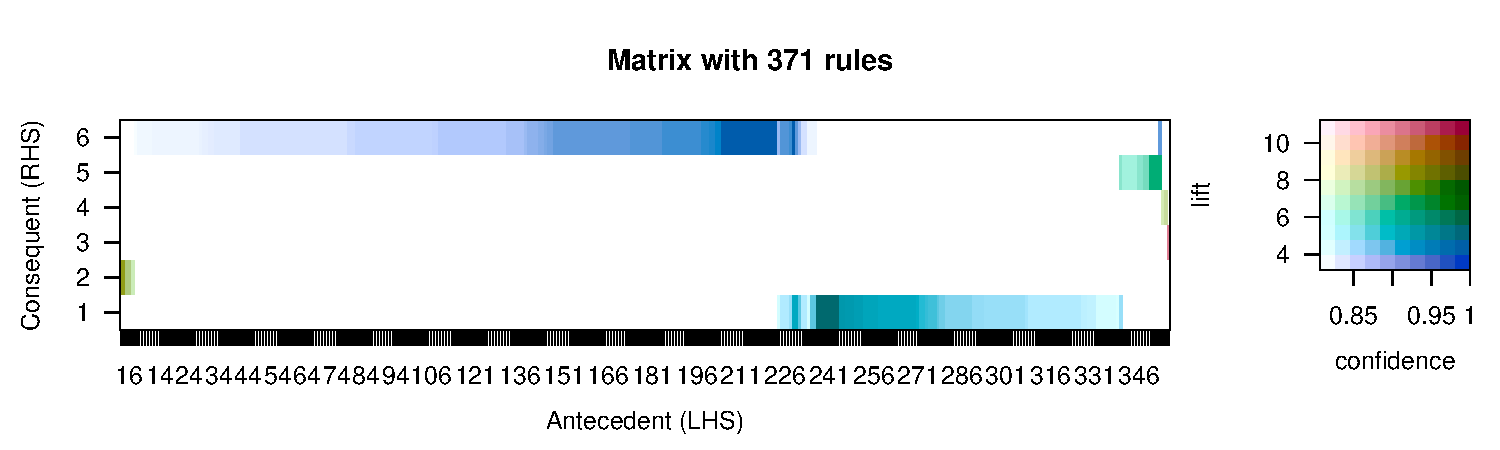
\includegraphics[width=\linewidth]{arulesViz-matrix_col2}
\caption{Matrix-based visualization of two measures with colored squares (reordered).
\label{fig:matrix_col2}}
\end{figure}

Figures~\ref{fig:matrix_col1} and \ref{fig:matrix_col2} show plots with two
measures of interest. The legend is here a color matrix.  By matching a square
with the closed color in the legend, we can determine both, support and
confidence.  High confidence/high support rules can be identified in the plot
as hot/red (high confidence) and dark/intense (high support).  Note that on a
black and white printout, the different colors are not distinguishable.



\section{Grouped matrix-based visualization}
\label{sec:grouped}

Matrix-based visualization is limited in the number of
rules it can visualize effectively
since large sets of rules typically also have large sets of
unique antecedents/consequents. Here we introduce a new visualization
techniques~\citep{arulesViz:Hahsler2011}
that enhances matrix-based visualization using grouping of rules
via clustering to handle a larger number of rules. Grouped rules
are presented as an aggregate in the matrix and can be explored
interactively by zooming into and out of groups.

A direct approach to cluster itemsets is to define a distance metric
between two itemsets $X_i$ and $X_j$.
A good choice is the Jaccard distance defined as

$$d_\mathrm{Jaccard}(X_i, X_j) = 1 -
\frac{|X_i \cap X_j|}{|X_i \cup X_j|}.$$

The distance simply is the number of items that $X_i$ and $X_j$ have in common
divided by the number of unique items in both sets.  For a set of $m$ rules we
can calculate the $m(m-1)/2$ distances and use them as the input for
clustering.  However, using clustering on the itemsets directly has several
problems. First of all, data sets typically mined for association rules are
high-dimensional, i.e., contain many different items. This high dimensionality
is carried over to the mined rules and leads to a situation referred is as the
``course of dimensionality'' where, due to the exponentially increasing volume,
distance functions lose their usefulness. The situation is getting worse
since minimum support used in association rule mining leads in addition to
relatively short rules resulting in extremely sparse data.

Several approaches to cluster association rules and itemsets to address the
dimensionality and sparseness problem were proposed in the literature.
\cite{arulesViz:Toivonen:1995}, \cite{arulesViz:Gupta:1999} and
\cite{arulesViz:Berrado:2007} propose clustering association rules by looking at
the number of transactions which are covered by the rules.
Using common covered
transactions avoids the problems of clustering sparse, high-dimensional binary
vectors. However, it introduces a strong bias towards clustering rules which
are generated from the same frequent itemset.  By definition of frequent
itemsets, two subsets of a frequent itemset will cover many common
transactions.  This bias will lead to mostly just rediscovering the already
known frequent itemset structure from the set of association rules.
%Yan 2005 suggests KL-divergence as distance between patterns.

Here we pursue a completely different approach.
We start with the matrix
$\mat{M}$
defined in Section~\ref{sec:matrix-based} which
contains the values of a selected interest measure of the rules
in set $\set{R}$. The columns/rows are the unique antecedents/consequents
in $\set{R}$, respectively.
Now grouping antecedents becomes the problem of grouping columns
in $\mat{M}$. To group the column vectors
fast and efficient into $k$ groups we use $k$-means clustering.
The default interest measure used is lift. The idea is that
antecedents that are statistically dependent on the same consequents
are similar and thus can be grouped together.
Compared to other clustering approaches for itemsets,
this method enables
us to even group antecedents containing substitutes
(e.g., butter and margarine)
which are rarely purchased together
since they will have similar dependence to the same consequents.

The same grouping method can be used for consequents. However,
since the mined rules
are restricted to a single item in the
consequent
there is no problem with combinatorial explosion and
such a grouping is typically not necessary.

To visualize the grouped matrix we use a balloon plot with antecedent
groups as columns and consequents as rows (see Figure~\ref{fig:clusterplot1}).
The color of the balloons
represent the aggregated interest measure in the group
with a certain consequent and the size of the balloon shows
the aggregated support. The default aggregation function is the median
value in the group. The number of antecedents
and the most important (frequent) items in the group are displayed
as the labels for the columns.
Furthermore, the columns and rows in the plot are reordered such that
the aggregated interest measure is decreasing from top down
and from left to right, placing the most interesting group in the
top left corner.

The matrix visualization with grouped antecedents
for the set of $5668$ rules mined earlier
can be easily created by
\begin{Schunk}
\begin{Sinput}
> plot(rules, method="grouped")
\end{Sinput}
\end{Schunk}

The resulting visualization is shown in Figure~\ref{fig:clusterplot1}.
The group of most interesting rules according to lift (the default measure)
are shown in the top-left corner of the plot. There are 3 rules
which contain ``Instant food products'' and up to 2 other items in the
antecedent and the consequent is ``hamburger meat.''

\begin{figure}
\centering
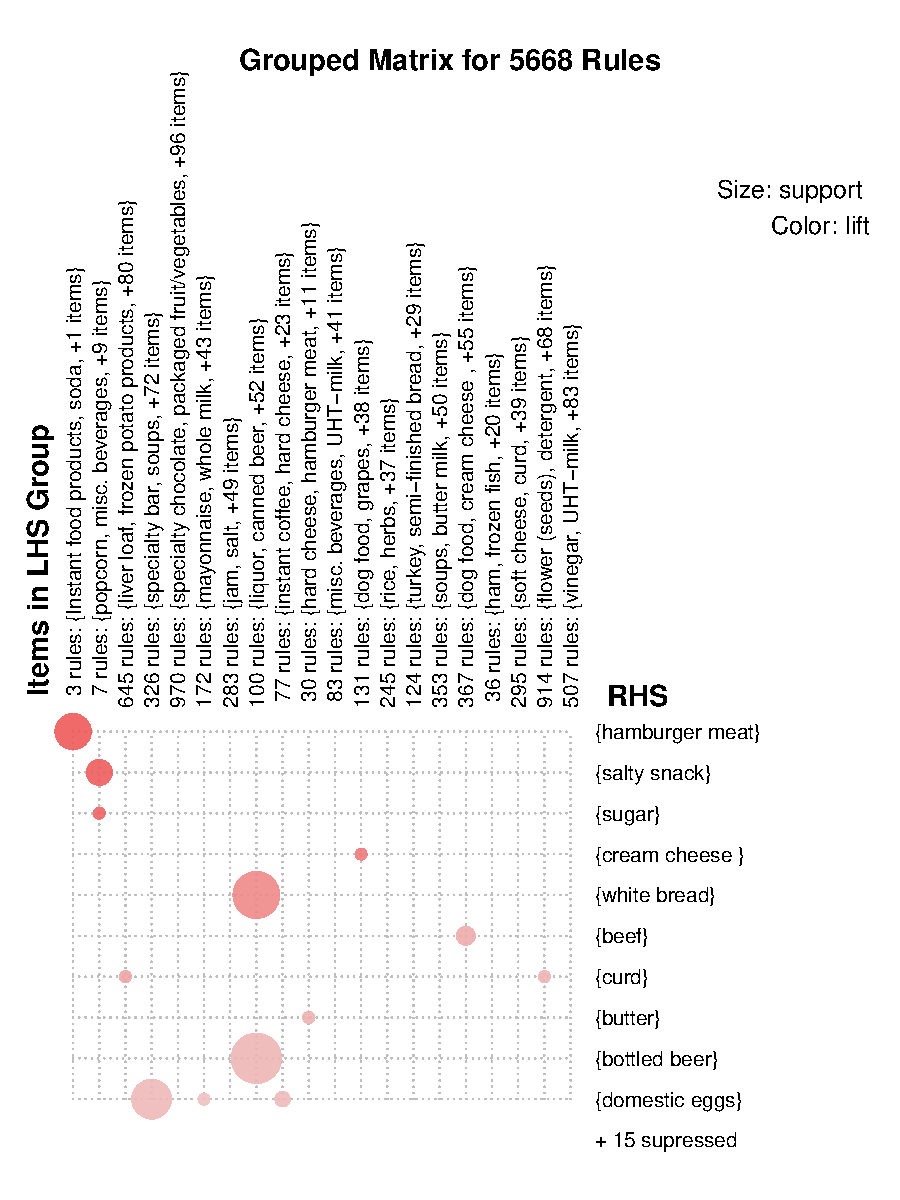
\includegraphics[width=12cm]{arulesViz-clusterplot1}
\caption{Grouped matrix-based visualization.\label{fig:clusterplot1}}
\end{figure}

To increase the number of groups we can change $k$ which defaults to 20.

\begin{Schunk}
\begin{Sinput}
> plot(rules, method="grouped", control=list(k=50))
\end{Sinput}
\end{Schunk}

The resulting, more detailed plot is shown in Figure~\ref{fig:clusterplot2}.

\begin{figure}
\centering
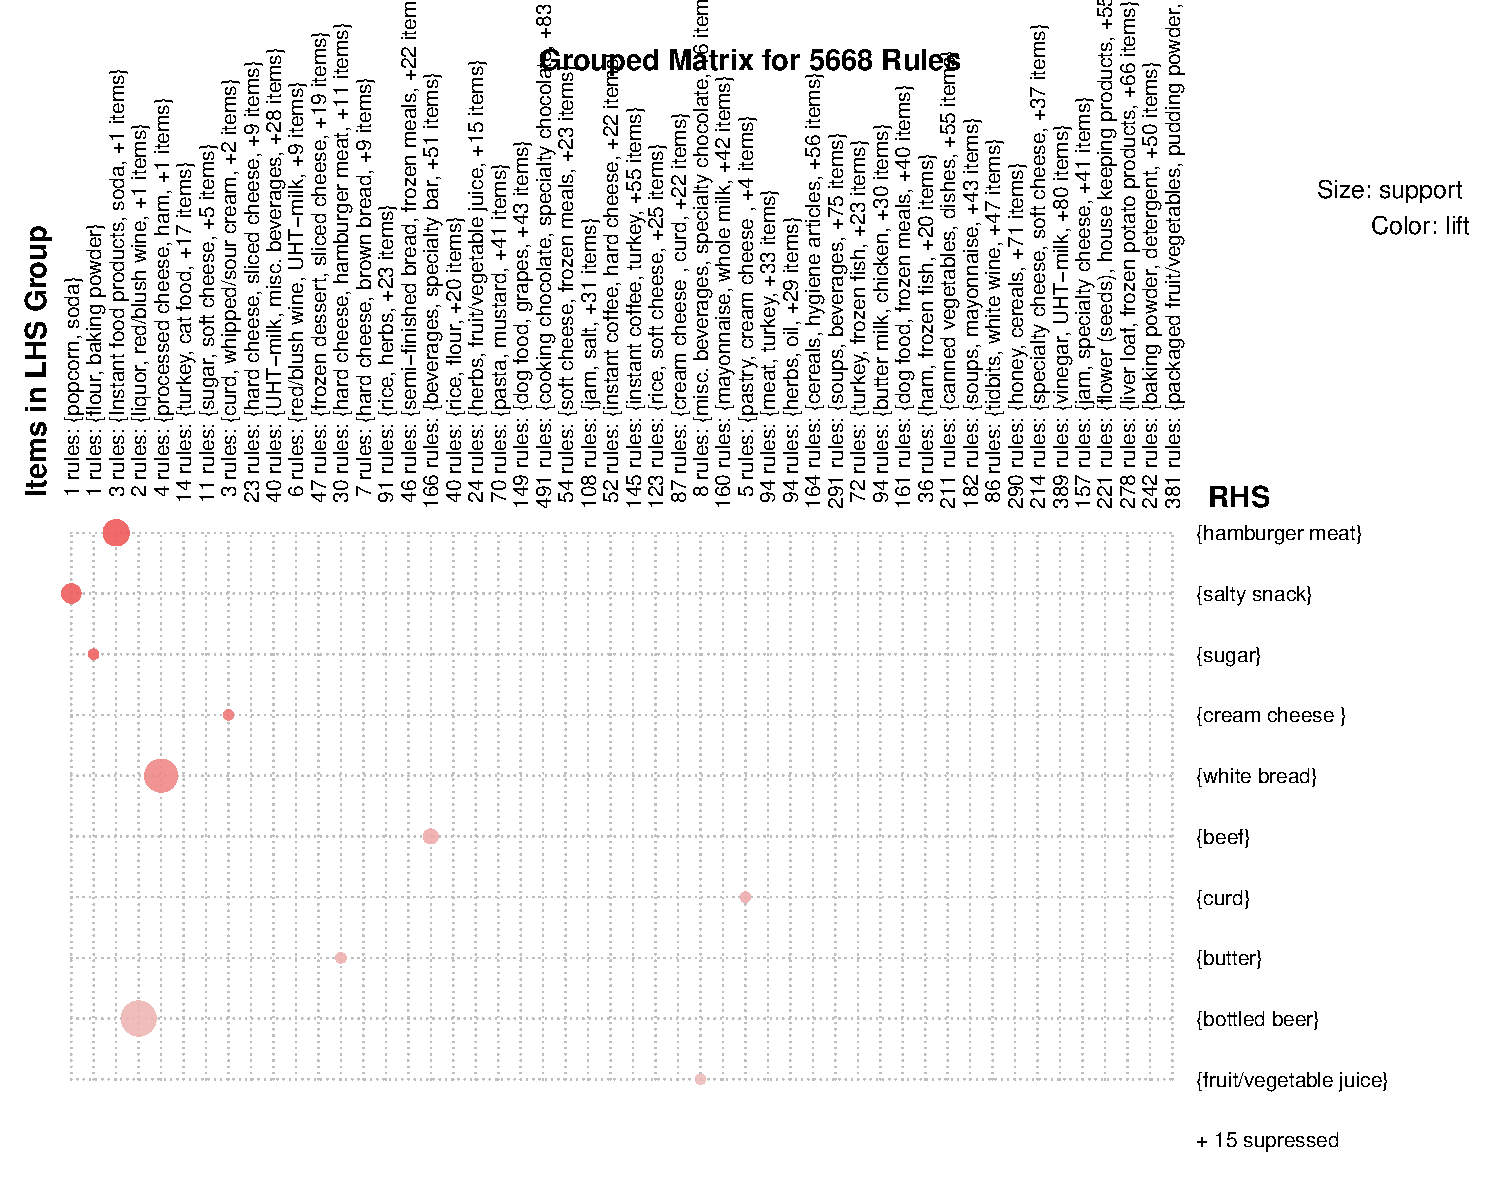
\includegraphics[width=20cm, angle=90]{arulesViz-clusterplot2}
\caption{Grouped matrix with $k=50$.\label{fig:clusterplot2}}
\end{figure}


An interactive version of the grouped matrix visualization is also available.

\begin{Schunk}
\begin{Sinput}
> sel <- plot(rules, method="grouped", interactive=TRUE)
\end{Sinput}
\end{Schunk}

Here it is possible to zoom into groups and to inspect
the rules contained in a selected group.

\section{Graph-based visualizations}

Graph-based techniques~\citep{arulesViz:Klemettinen:1994,arulesViz:Rainsford:2000,arulesViz:Buono:2005,arulesViz:Ertek:2006} visualize association rules
using vertices and edges where vertices typically represent items
or itemsets and edges indicate relationship in rules. Interest measures are
typically added to the plot as labels on the edges or by color or width of
the arrows displaying the edges.

Graph-based visualization offers a very clear representation of rules but they
tend to
easily become cluttered and thus are only viable for very small sets of rules.
For the following plots we select the 10 rules with the highest lift.

\begin{Schunk}
\begin{Sinput}
> subrules2 <- head(sort(rules, by="lift"), 10)
\end{Sinput}
\end{Schunk}

\pkg{arulesViz} contains several graph-based visualizations
rendered using
either the \emph{igraph} library via package
\pkg{igraph}~\citep{arulesViz:Csardi2006}
or
the interface to the \emph{GraphViz} software in
package \pkg{Rgraphviz}~\citep{arules:Gentry:2010}.
By default igraph is used.
The following
plot represents items and rules as vertices connecting them with directed edges
(shown in Figure~\ref{fig:graph1}).

\begin{Schunk}
\begin{Sinput}
> plot(subrules2, method="graph")
\end{Sinput}
\end{Schunk}

\begin{figure}
\centering
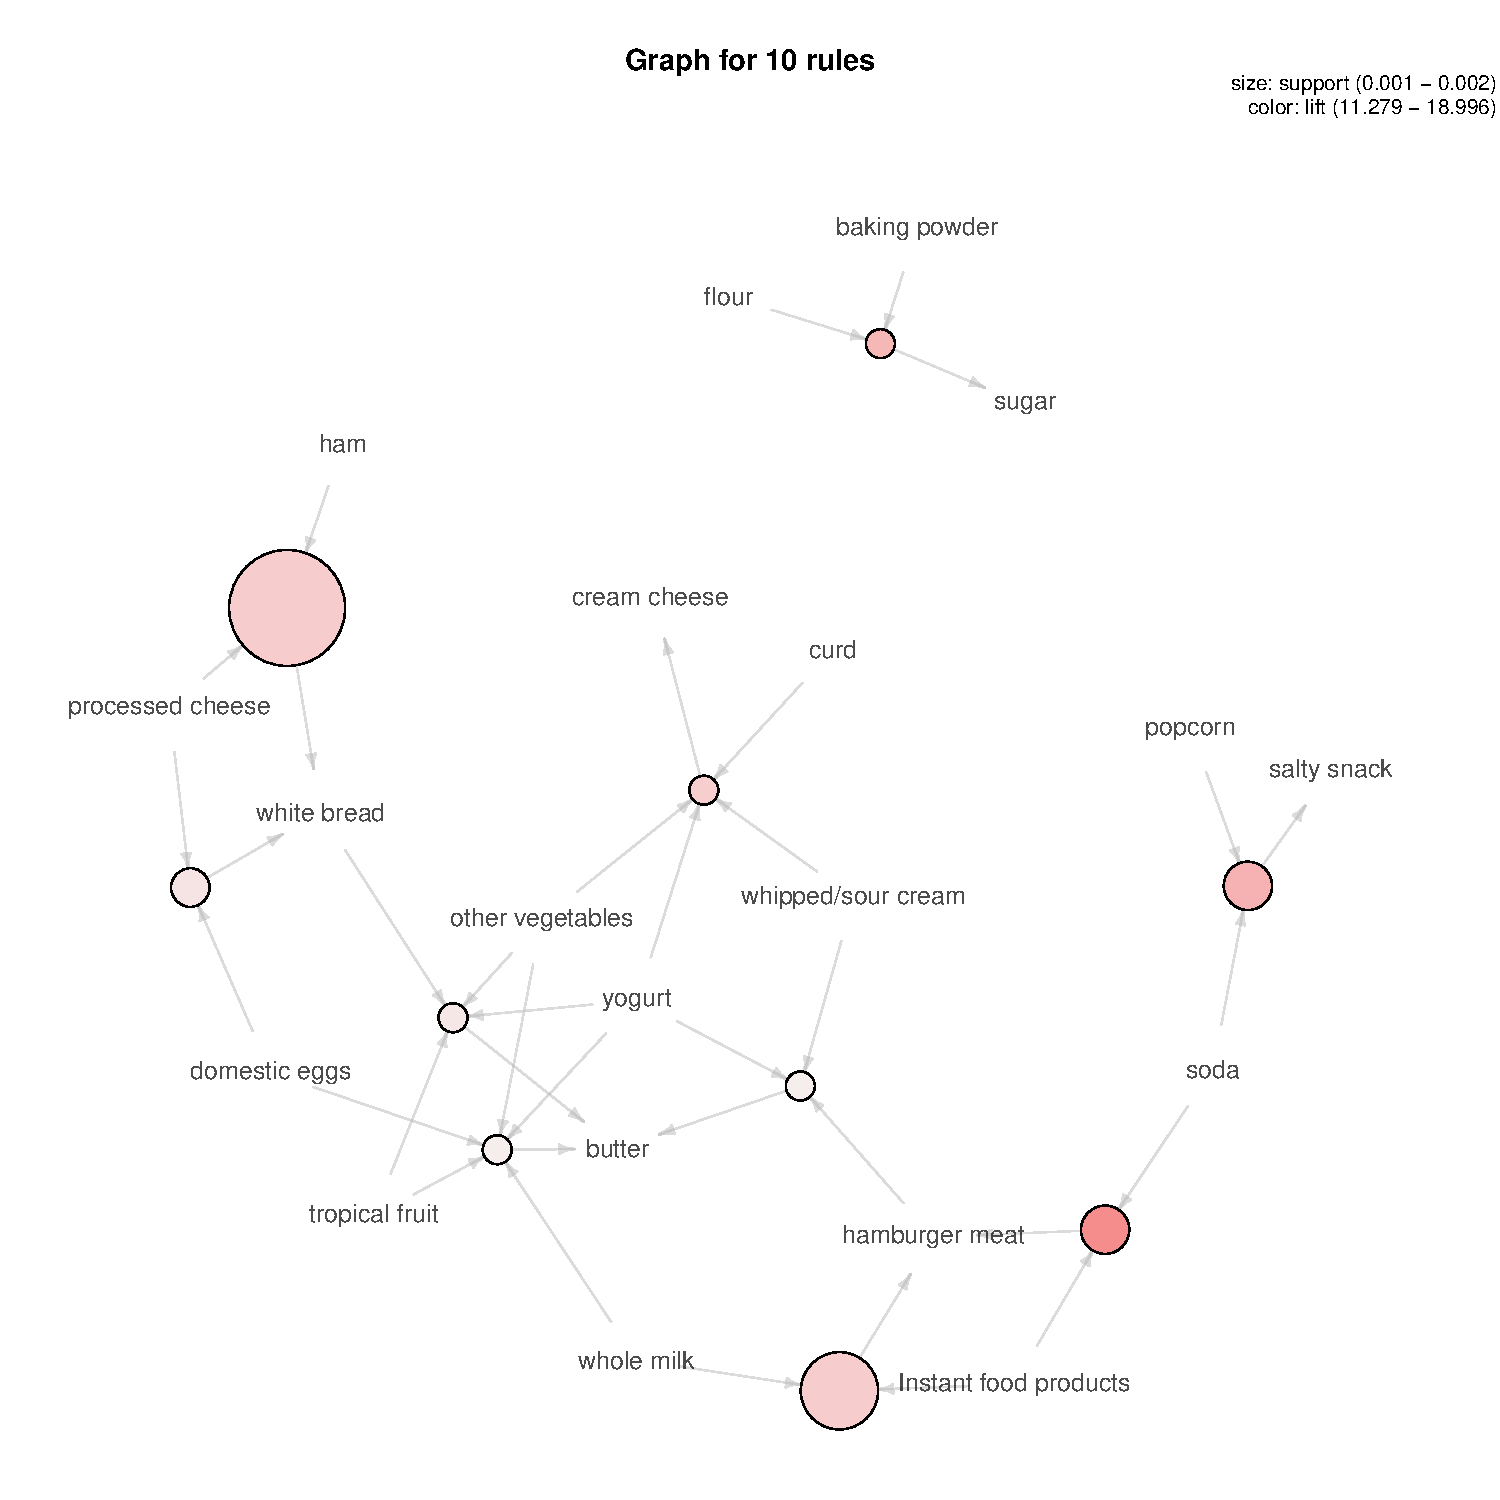
\includegraphics[width=\linewidth]{arulesViz-graph1}
\caption{Graph-based visualization with items and rules as vertices.
\label{fig:graph1}}
\end{figure}


Another variation uses itemsets as vertices and rules are represented by
directed edges.

\begin{Schunk}
\begin{Sinput}
> plot(subrules2, method="graph", control=list(type="itemsets"))
\end{Sinput}
\end{Schunk}

\begin{figure}
\centering
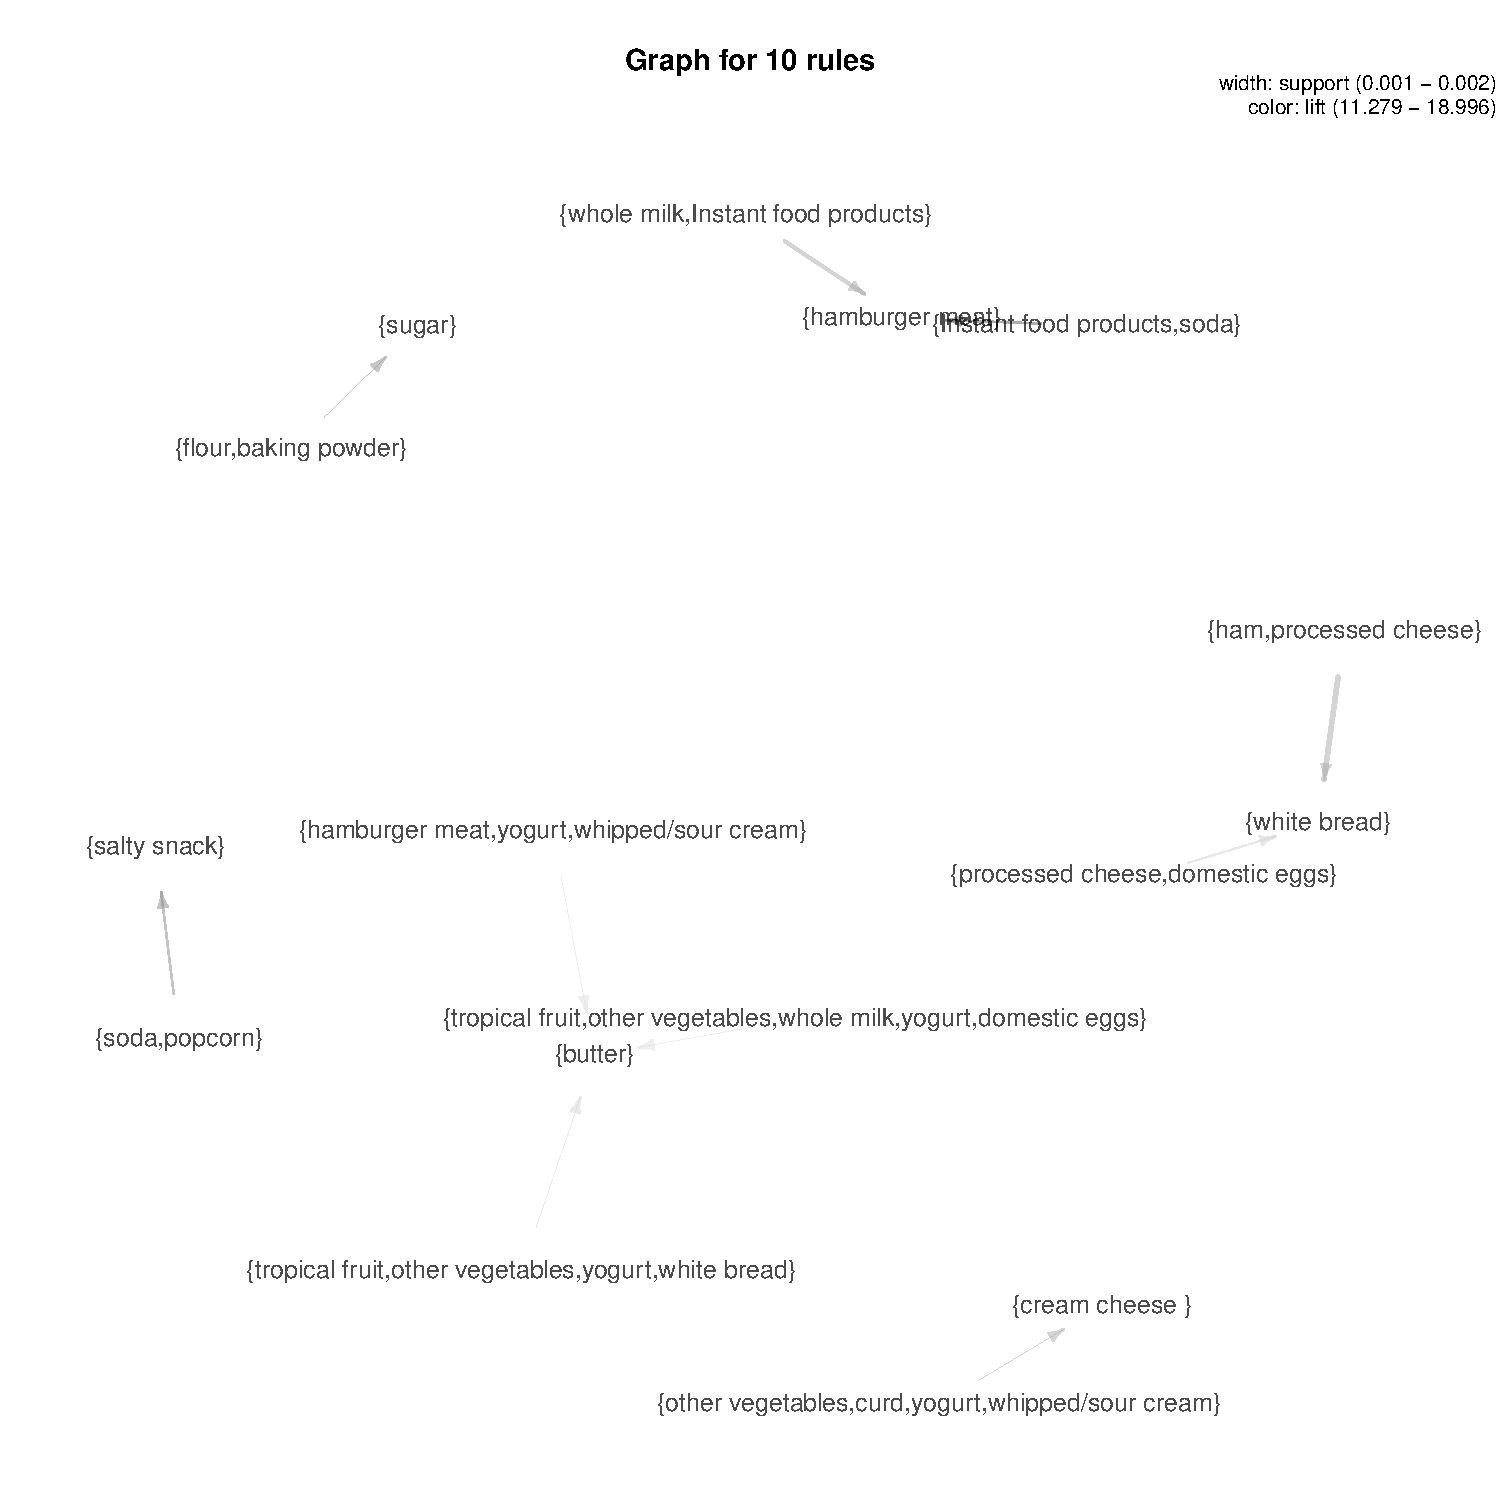
\includegraphics[width=\linewidth]{arulesViz-graph3}
\caption{Graph-based visualization with itemsets as vertices.
\label{fig:graph3}}
\end{figure}

Figure~\ref{fig:graph3} shows the resulting graph.
This representation focuses on how the rules are composed of individual items
and shows which rules share items.

An interactive visualization is available in \pkg{arulesViz},
however,
the built-in graph based visualizations are only
useful for small set of rules.  To explore large sets of rules with graphs,
advanced interactive features like zooming, filtering, grouping and coloring
nodes are needed. Such features are available in interactive visualization
and exploration platforms for
networks and graphs like \emph{Gephi}~\citep{arules:Bastian:2009}.
From \pkg{arulesViz} graphs for sets of association rules can be exported
in the GraphML format
or as a Graphviz dot-file
to be explored in tools like Gephi. For example the
1000 rules with the highest lift are exported by:

\begin{Schunk}
\begin{Sinput}
> saveAsGraph(head(sort(rules, by="lift"),1000), file="rules.graphml")
\end{Sinput}
\end{Schunk}

Figure~\ref{fig:gephi} shows a screenshot of exploring these rules
interactively. Rules can be explored by zooming, filtering and coloring
vertices and edges.

\begin{figure}
\centering
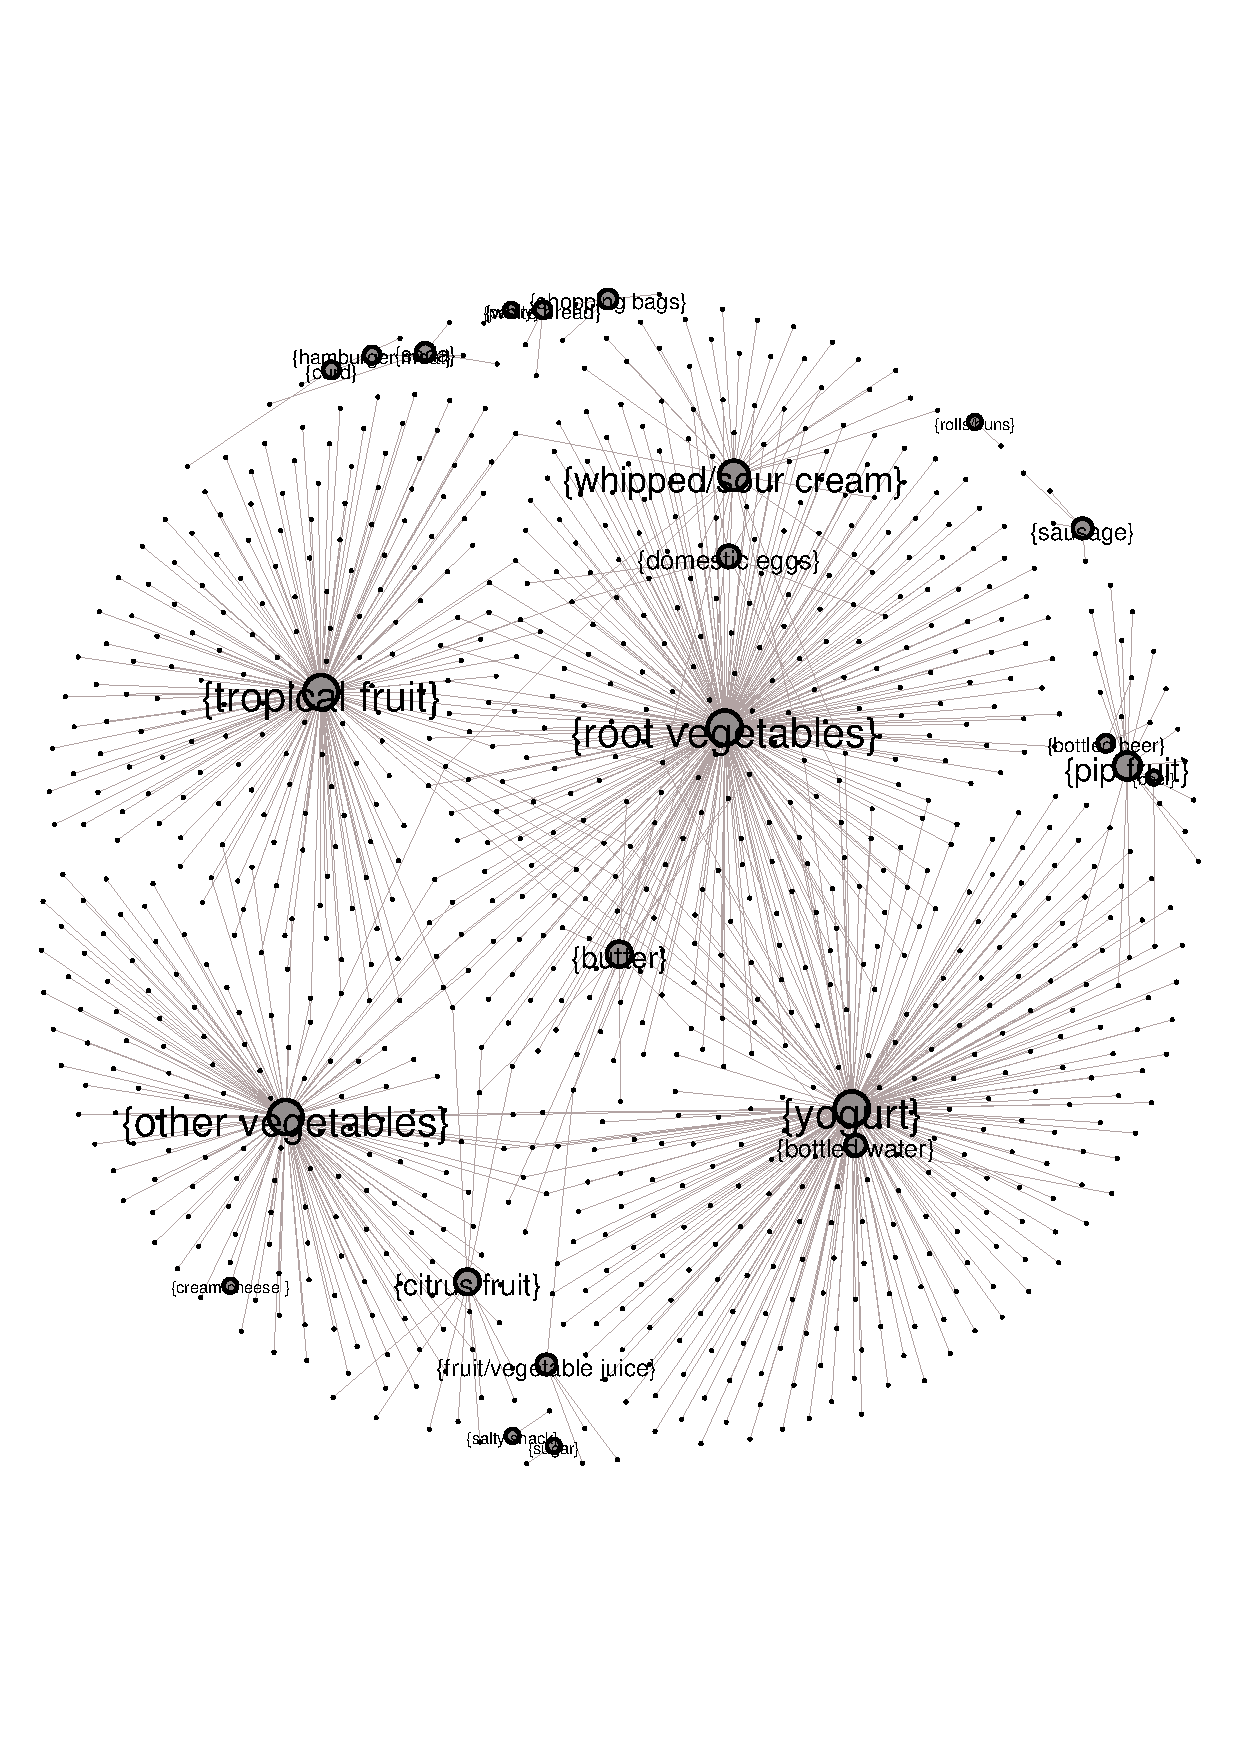
\includegraphics[width=\linewidth]{gephi_1}
\caption{Visualization of 1000 rules with Gephi (Fruchterman Reingold layout, vertex and label size is proportional to the in-degree, i.e., the number of
rules the consequent participates in).
\label{fig:gephi}}
\end{figure}


\section{Parallel coordinates plot}

Parallel coordinates plots are designed to visualize multidimensional data
where each dimension is displayed separately on the x-axis and the
y-axis is shared. Each data point is represented by a line
connecting the values for each
dimension.
%%% MFH: what does the following mean?
Parallel coordinates plots were used previously to visualize
discovered classification rules \citep{arulesViz:cviz}
and association rules \citep{arulesViz:Yang:2003}. \cite{arulesViz:Yang:2003}
displays the items on the y-axis as nominal values and the x-axis represents
the positions in a rule, i.e., first item, second item, etc.  Instead of a
simple line an arrow is used where the head points to the consequent item.
Arrows only span enough positions on the x-axis to represent all the items in
the rule, i.e., rules with less items are shorter arrows.

\begin{Schunk}
\begin{Sinput}
> plot(subrules2, method="paracoord")
\end{Sinput}
\end{Schunk}

Figure~\ref{fig:pc1} shows a parallel coordinates plot for 10 rules.
The width of the arrows represents support and the intensity of the color
represent confidence.
It is obvious that
for larger rule sets
visual analysis
becomes difficult since with an increasing number of rules also
the number of crossovers
between the lines increases \cite{arulesViz:Yang:2003}.

The number of crossovers can be significantly reduced by reordering the items
on the y-axis. Reordering the items to minimize the number of
crossovers is a combinatorial problem with $n!$ possible permutations.
However, for visualization purposes a suboptimal but fast solution is
typically acceptable. We applies a variation of the well known
2-opt heuristic
\cite{arulesViz:Bently:1990} for travelers salesman problem
to the reordering problem. The objective function is to minimize the
number of crossovers. The simple heuristic uses the following steps:
\begin{enumerate}
\item Choose randomly two items and exchange them if it improves the
objective function.
\item Repeat step 1 till no improvement is found for a predefined number
of tries.
\end{enumerate}

Reordering is achieved with \code{reorder=TRUE}.
\begin{Schunk}
\begin{Sinput}
> plot(subrules2, method="paracoord", control=list(reorder=TRUE))
\end{Sinput}
\end{Schunk}

Figure~\ref{fig:pc2}
shows the parallel coordinates plot with reordered items
to reduce crossovers.

\begin{figure}
\centering
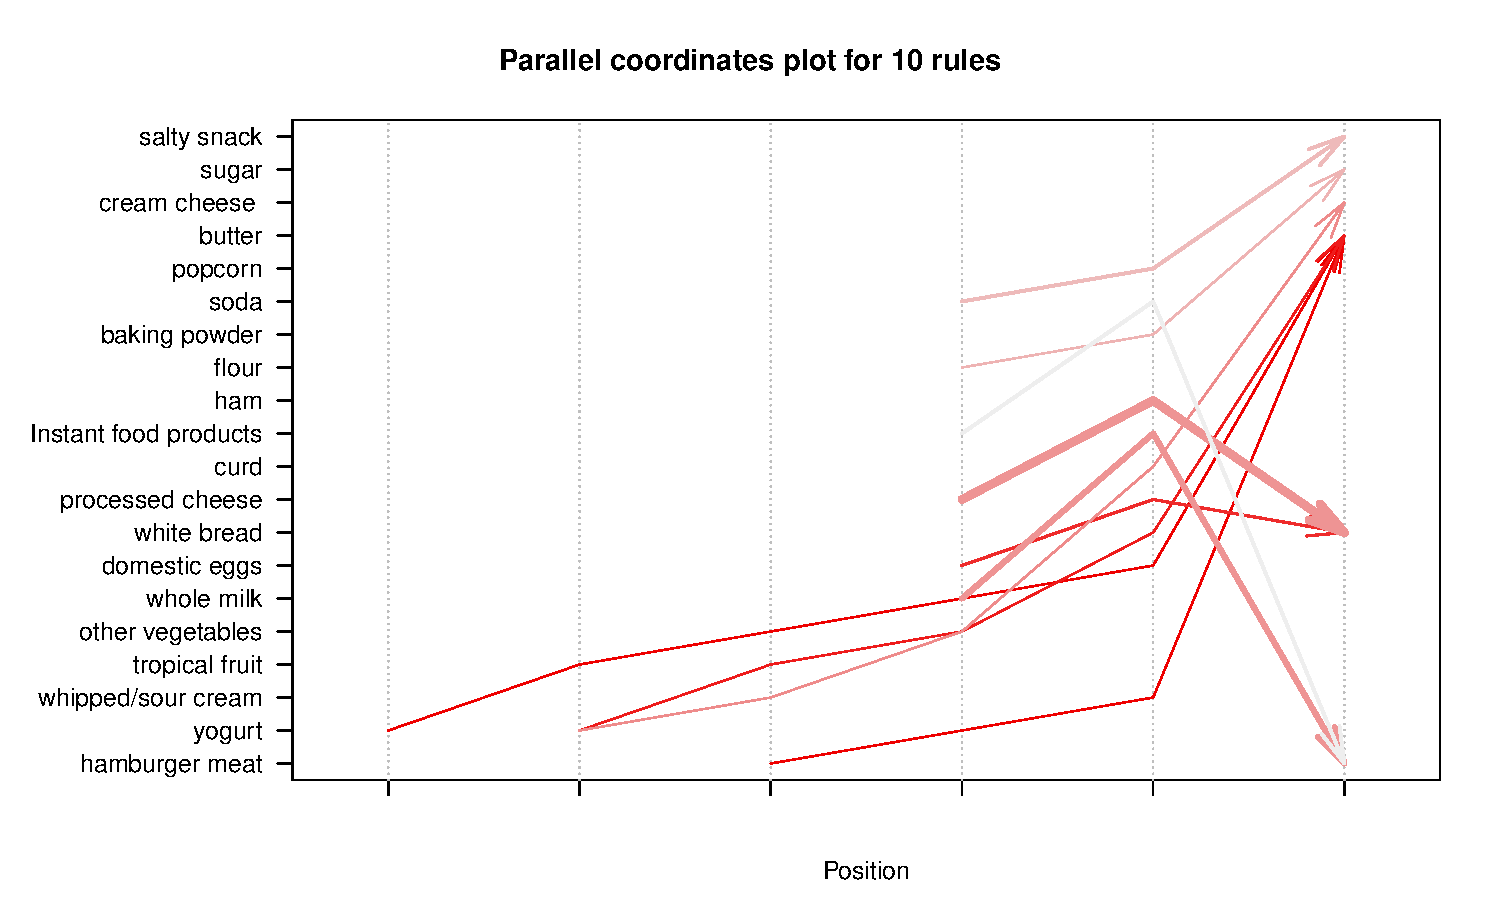
\includegraphics[width=15cm]{arulesViz-pc1}
\caption{Parallel coordinate plot.\label{fig:pc1}}

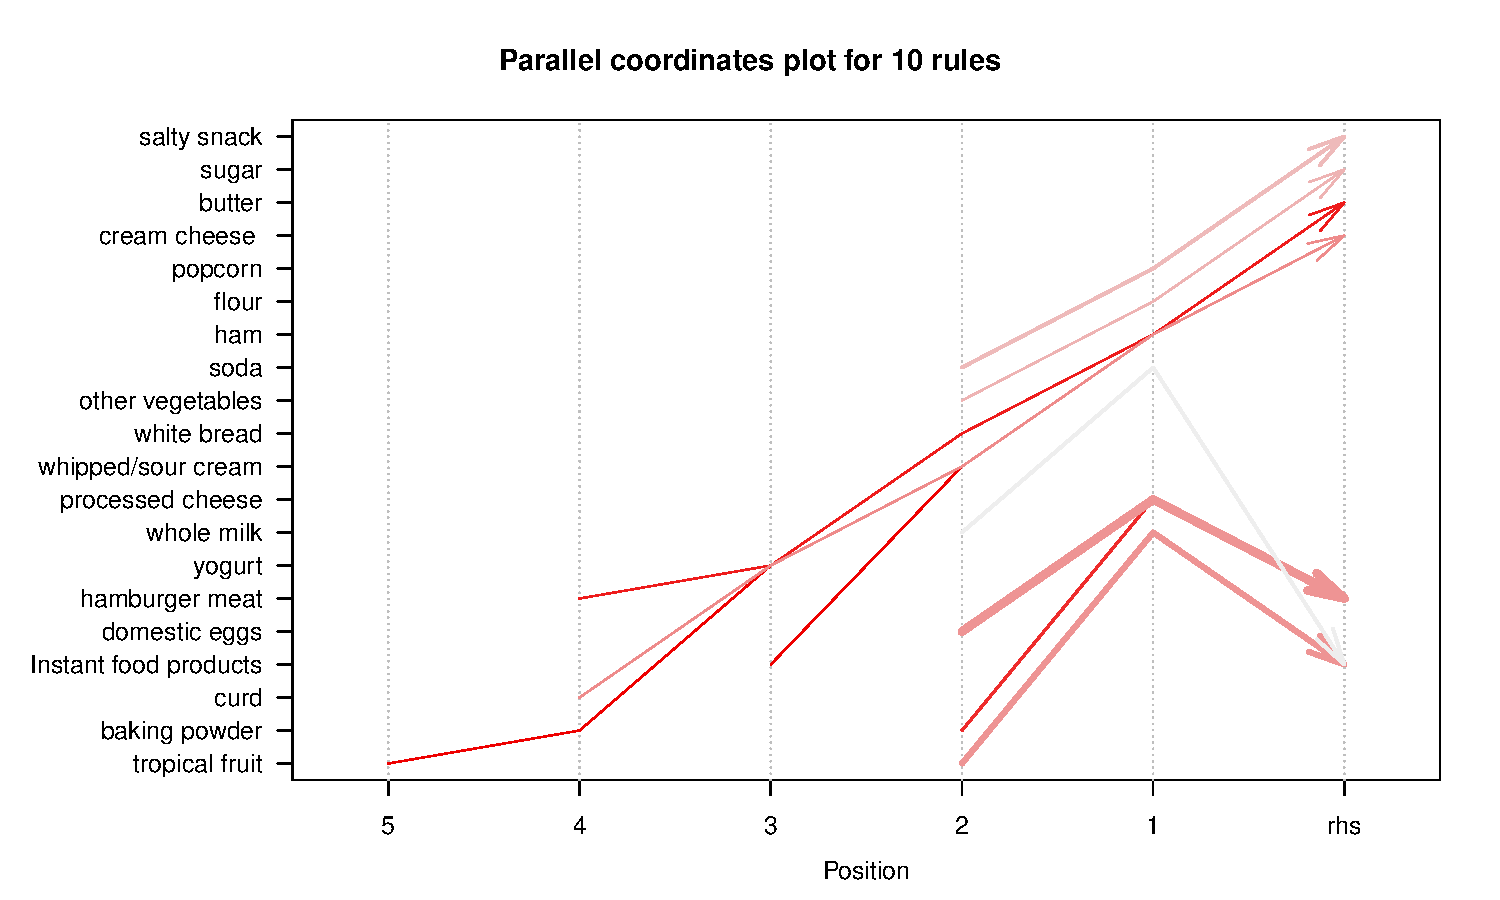
\includegraphics[width=15cm]{arulesViz-pc2}
\caption{Parallel coordinate plot (reordered).\label{fig:pc2}}
\end{figure}

\section{Double Decker plots}
\label{sec:doubledecker}

A double decker plot is a variant of a mosaic plot.  A mosaic plot
displays a contingency table using tiles on a rectangle created by recursive
vertical and horizontal splits. The size of each tile is proportional to the
value in the contingency table. Double decker plots use
only a single horizontal split.

\cite{arulesViz:Hofmann:2000} introduced
double decker plots to visualize a single association rule.
Here the displayed contingency table is computed for a rule by counting
the occurrence frequency for each subset of items in the antecedent and
consequent from the original data set.
The items in the antecedent are used for the vertical splits
and the consequent item is used for horizontal highlighting.

We randomly choose a single rule and visualize it with a double decker plot.
\begin{Schunk}
\begin{Sinput}
> oneRule <- sample(rules, 1)
> inspect(oneRule)
\end{Sinput}
\begin{Soutput}
    lhs                           rhs                support    
[1] {citrus fruit,butter,soda} => {other vegetables} 0.001016777
    confidence lift    
[1] 0.625      3.230097
\end{Soutput}
\end{Schunk}

\begin{Schunk}
\begin{Sinput}
> plot(oneRule, method="doubledecker", data = Groceries)
\end{Sinput}
\end{Schunk}
\begin{figure}
\centering
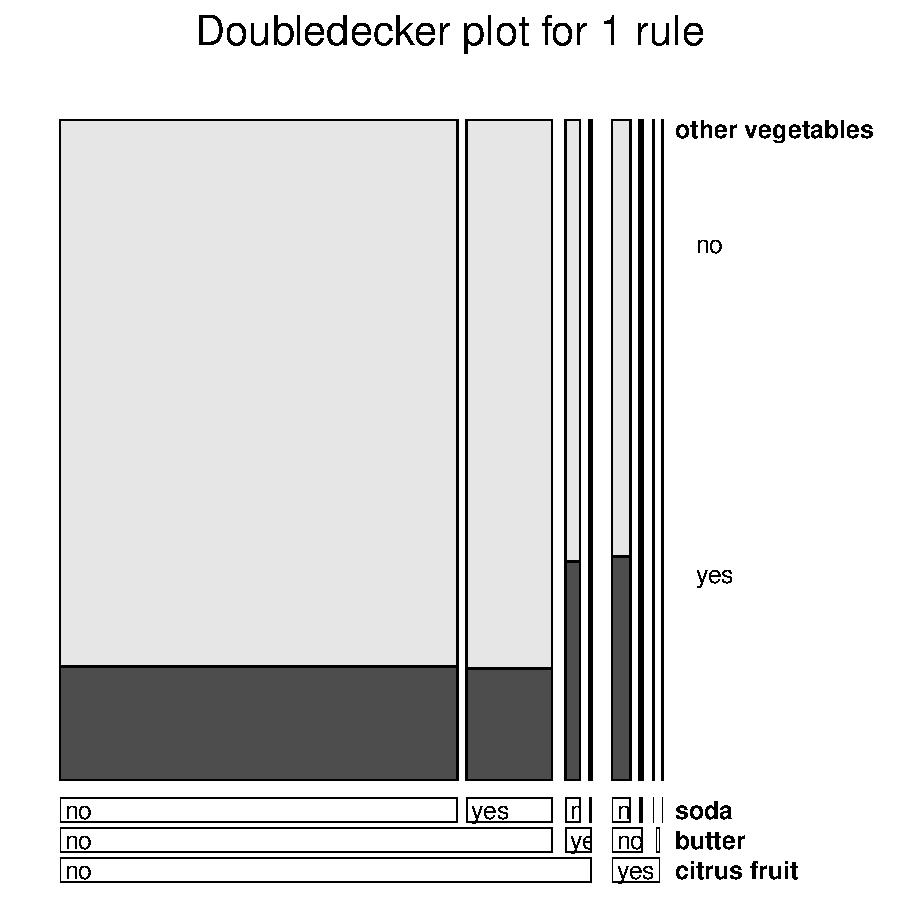
\includegraphics[width=8cm]{arulesViz-doubledecker1}
\caption{Double decker plot for a the rule
{citrus fruit,butter,soda} => {other vegetables}.\label{fig:doubledecker1}}
\end{figure}

Figure~\ref{fig:doubledecker1} shows the resulting plot.
The area of blocks gives the support and the height of the ``yes'' blocks is
proportional to the confidence for the rules consisting of the antecedent items
marked as ``yes.''
Items that show a significant jump in confidence when changed from
``no'' to ``yes'' are interesting. This is captured
by the interest measure \emph{difference of confidence} defined by
\cite{arulesViz:Hofmann:2001}.

%%% MFH: difference of confidence
%%% MFH: \marginpar{order of antecedents}

\section{Comparison of techniques}
\label{sec:comp}

In this section, we compare the visualization techniques
available in \pkg{arulesViz}
based on the size of the rule set
which can be analyzed, the number of interest measures which are shown
simultaneously,
if the technique offers interaction and reordering
and how intuitive each visualization technique is. Note that most of these
categories are only evaluated qualitatively here, and the results
presented in Table~\ref{tab:comp}
are only meant to guide the user towards the most suitable techniques for
a given application.

Scatterplot (including two-key plots) and grouped matrix plot are capable to
analyze large rule sets. These techniques are interactive to allow
the analyst to zoom and select interesting rules. Matrix-based
can accommodate rule sets of medium size. Reordering can be used to improve
the presentation.
To analyze small rule sets the matrix-based method with 3D bars,
graph-based methods and parallel coordinates
plots are suitable. Graphs for large rule sets can be analyzed using
external tools like Gephi.
Finally, double decker plots only visualize a single rule.

The techniques discussed in this paper can also be
categorized based on the number of interest measures simultaneously
visualized. Most methods can represent two measures and scatter plots
are even able to visualize three measures for each rule in one plot.

Scatter plot and graph based techniques are the most intuitive while
matrix-based visualization with two interest measures, parallel coordinates
and double decker require time to learn how to interpret them correctly.

%%% MFH: add fpvat
%\cite{arulesViz:Carson:2010}, provides good interactive tool for association
%rules to zoom and select and it supports reordering also.

\begin{table}
\centering
{\footnotesize
\begin{tabular}{l@{  }l@{  }c@{  }c@{  }c@{  }c@{  }c}
\hline
{\bf Technique} & {\bf Method} & {\bf Rule set} & {\bf Measures} & {\bf Interactive} & {\bf Reordering} & {\bf Ease of use}\\
\hline
Scatterplot& \tt "scatterplot" & large & 3 & \checkmark &  & ++ \\
Two-Key plot & \tt "scatterplot" & large & 2 + order & \checkmark &  & ++ \\
Matrix-based  & \tt "matrix" & medium & 1 & & \checkmark & 0\\
Matrix-b. (2 measures) & \tt "matrix" & medium & 2 & &  \checkmark & -- --\\
Matrix-b. (3D bar) & \tt "matrix3D" &  small & 1 & &  \checkmark & +\\
Grouped matrix & \tt "grouped" &  large & 2 & \checkmark &  \checkmark & 0\\
Graph-based &  \tt "graph" & small & 2 & & & ++\\
Graph-b. (external) &  \tt "graph" & large & 2 &  \checkmark &  \checkmark & +\\
Parallel coordinates & \tt "paracoord" & small & 1 & & \checkmark & --\\
Double decker & \tt "doubledecker" & single rule & (2) & & & --\\
\hline
\end{tabular}
\caption{Comparison of visualization methods for association rules available in
\pkg{arulesViz}.\label{tab:comp}}
}
\end{table}

%
%      \begin{figure}
%      \centering
%      \renewcommand{\arraystretch}{1.2}
%{\footnotesize
%    \begin{tabular}{|l|l|l|p{2.5cm}|}
%    \hline
%    {\bf Method Name} & {\bf Name } & {\bf Figuare 4 } & {\bf Limitation}\\
%    \hline
%        Graph & Graph & - & Limited to Small Number of Itemsets \\
%        Parallel Coordinates & Parallel Coordinates & (g) & Limited to Small Number of Itemsets \\
%        \hline
%        \end{tabular}}
%        \caption{Comparison of Visualization Methods for Itemsets.\label{table:itemcompvistech1}}
%        \end{figure}
%
%

%
%From Tables ~\ref{table:compvistech} and ~\ref{table:itemcompvistech1}, all the methods are limited to one rule or some number of rules this is due to complexity in representation. As mentioned earlier association rule mining algorithms typically generate a large number of rules, matrix shading and cluster plot visualization techniques can accommodate more number of rules when compared to other techniques with this feature matrix shading and cluster plot visualization techniques could be the most effective among all.
%

%\section{To Improve Visualization}
%Visual representations are needed to facilitate exploratory analysis, but there are some difficulties in understanding the visual information in overcrowded and cluttered displays. So, to incorporate more number of rules and to avoid crossover/cluttering problems we are using two types of improvement techniques, one is reodering the items and the other is clustering the items. With this reordering and clustering methods the analyst can only inspect or analyze rules which are interesting.
%
%\subsection{Reordering Items}
%The above mentioned problems are caused due to the unorderedness of data, mostly the data we are using for visualization is not ordered. Basically, data analysis had a problem in arranging the objects to reveal structural information. From \citep{arulesViz:seriate}, they defined this problem as seriation and also proposed methods to overcome the seriation or sequencing problem. As discussed earlier ordering or organising the data can greatly imporve the quality of visualization.
%We integrated these seriation methods with some of our visualization techniques to understand the data in efficient way. We can not apply these seriation methods to all of our techniques since we are preprocessing the generated data differently for each of the visualization techniques. So, to avoid the overcrowded and cluttered displays for other techiniques we ordered the data by sorting or rearranging the data items.
%We applied these seriation methods to matrix shading technique to analyze the rules in more understanding way. As we are using matrix data structure to represent the data, so we applied some seriation methods discussed in \citep{arulesViz:seriate} and after convincing results we extended our work in using and designing ordering methods, which improved the quality of data representation.
%
%\subsection{Clustering Items}
%Too many rules cause overlapping problem for visual interpretation, which is due to limited space. Clustering can help in visualizing and ordering the items, by reducing the large number of association rules \citep{arulesViz:clusrules}, which is achieved by  clustering the rules based on quantitative attributes. For example the rules \{$age=16 \Rightarrow salary=0$\} and \{$age=17 \Rightarrow salary=0$\} after clustering the antecedent items based on consequent, now the rule changed as \{$17<age>16 \Rightarrow salary=0$\}. \citep{arulesViz:disclus}, they are clustering the association rules based on the distance metric and the distance could be found from the quality measures like support, confidence, etc,.
%This clustering can be applied to 3D matrix and cluster plot. As we are using this clustering to accomodate more number of rules and also to find which of the consequent items have the similar antecedent items.
%



\section{Conclusion}
\label{sec:conclusion}

Association rule mining algorithms typically generate a large number of
association rules which poses a major problem for understanding and analyzing
rules.  In this paper we presented several visualization techniques
implemented in \pkg{arulesViz} which can be used to explore and present
sets of association rules.
In addition we present a new interactive visualization method called
grouped matrix-based visualization which can used to effectively
explore large rule sets.

Future development will focus on
enhancing the visualizing techniques with advanced interactive features
using for example \pkg{iplots}~\citep{arulesViz:Urbanek:2003}
which supports in addition to selection and zooming
also brushing and linking between different plots.

%\bibliographystyle{abbrvnat}
\bibliography{arulesViz,arules}


\end{document}

